\chapter{Introduction}
\label{ch:Intro}


%%%%%%%%%%%%%%%%%%%%%%%%%%%%%%%%%%%%%%%%%%%%%%%%%%


\section{Psoriasis and psoriatic arthritis}
%
Psoriasis and psoriatic arthritis (PsA) have been described as two different common complex disease entities. Psoriasis is a chronic inflammatory dermatose disease with episodes of relapse and remittance \parencite{Nestle2009}. On the other hand, PsA is a seronegative chronic inflammatory disease within the family of spondyloarthritis \parencite{Moll1973, Coates2016} that usually develops after psoriasis skin manifestations\parencite{Villanova2016}. Psoriasis and PsA are distinct disease conditions that share nonetheless certain clinical features and genetic architecture. The study of those similarities and differences at the pathological and genetic levels will benefit the understanding of genetic variability in the risk to develop psoriasis and PsA as well as the identification of new therapeutic targets.

%(Variants in RUNX3 contribute to susceptibility to PsA, exhibiting further common ground with ankylosing spondylitis, PsA Immunochip)

\subsection{Epidemiology and global impact}
%
Psoriasis represents a serious global health problem that currently affects about 100 million people worldwide, including children and adults with no sex bias \parencite{Organization2016}. Alike the minor correlation with geographic latitude, the development of psoriasis presents a strong ethnicity component \parencite{Jacobson2011}. In fact, the prevalence of psoriasis in adults is lower among African, African American and Asian (between 0.4 and 0.7\%) compared to American and Canadian populations (4.6 and 4.7\%, respectively). In the UK, psoriasis prevalence ranges between 2 and 3\%, affecting approximately 1.8 million of people \parencite{Perera2012}.

On the other hand, the cases of PsA in the general population varies between 0.04 and1.2\% \parencite{Perera2012} but dramatically increase up to 10 to 30\% within psoriasis patients \parencite{Gelfand2005,Reich2008}, evidencing the strong association between the two diseases. Particularly, in the UK, 14\% of the psoriasis patients develop chronic inflammatory arthritis in the form of PsA during the course of the disease \parencite{Ibrahim2009}. Overall, data suggest an steady increase in both, psoriasis and PsA, prevalence over time \parencite{Springate2007,Organization2016}.


Although psoriasis can be developed at any age, onset of disease seems to have a bimodal distribution strongly influenced by the Human Leukocyte Antigen (HLA) Cw*06:02 (HLA-Cw6:02), an allele for one of the genes in the Major Histocompatibility Complex (MHC) I, involved in antigen presentation \parencite{Henseler1985} and the strongest genetic association with psoriasis and PsA risk \parencite(Ellinghaus2010, Strange2010, Stuart2010; Sun2010). The early-onset or Type I is characterised by development of disease around 16-22 and 30-39 years and a prevalence for HLA-C*06:02 (85.4\% of the cases). In contrasts, the late-onset or Type II group manifests disease between 50-60 years old and presents positive HLA-C*06:02 only in 14.6\% of the cases. %This classification based on the age of onset has also correlates with distinctive clinical clinical features including severity, relapse frequency and family history.

Accordingly, psoriasis and PsA represent a burden for the countries' economies due to treatment’s costs and associated morbidity.  In the UK treatment and management-associated costs for psoriasis in 2015 accounted for £4,000 to £14,000, before and after requirements of biological therapy, respectively \parencite{Burgos-Pol2016, Poole2010} and the costs are further enhanced in the case of PsA.



\subsection{Psoriasis and inflammatory dermatoses}
%

The group of inflammatory dermatoses affects up to 70\% of the population and it represents the 4$^{th}$ leading cause of nonfatal burden \parencite{ICD-10,Roderick2014}. The skin is the biggest organ in the human body constituting an effective barrier between the environment and the internal organs. The most external layer, the epidermis, plays a relevant role in the innate and adaptive immunity and its alterations, due to exogenous or endogenous factors, can lead to development of inflammatory dermatose conditions such as psoriasis or atopic dermatitis (AD) \parencite{Johnson-Huang2009, Proksch2008}}. Lesions in psoriasis are very heterogeneous in type (pustular and non-pustular), location and severity, which difficult its clinical classification \parencite{Perera2012}. As a result, several phenotypes including psoriasis vulgaris, guttate, pustular, erythroderma and nail pitting have been defined and it is under debate whether some of those should be considered independent disease entities \parencite{Marrakchi2011}.


\subsection{PsA and spondyloarthropaties}
%
PsA belongs to the family known as spondylarthropaties (SpA) which includes phenotypes such as ankylosing spondylitis (AS), reactive arthritis (ReA), idiopathic inflammatory bowel disease (IBD) and undifferentiated SpA \parencite{Baeten2013}. All these SpA subtypes are characterised by structural damage (bone formation and erosion) as well as inflammation of joints and extra-articular sites such as eyes, gut and skin. Broadly, SpA has been classified into axial and peripheral base on the affected joints (spine/sacroilicac or peripheral) and the presence of extra-articular features \parencite{Runwaleit2001, Runwaleit2001}. Studies in human families and rat models with HLA-B27 positive status have shown manifestation of different SpA forms, such as psoriasis and inflammatory bowel disease (IBD), within a single family or individual \parencite{Hammer1990,Said-Nahal2000}. These observations support the hypothesis that SpA subtypes may be a single multifaceted condition with shared genetic, immunophatological and structural features and dynamic phenotypes \parencite{Baeten2013}. Conversely, some studies suggest that the immunopathological differences between axial and peripheral arthritis could be partially explained by genetic factors \parencite{Porcher2005, Appel2011, Noordenbos2012}.

As a phenotype, PsA can be further subdivided in five clinical groups as per Moll and Wright criteria: distal, destructive, symmetric, asymmetric and spinal \parencite{Moll1973}. These subclasses mainly differ in the location, number and distribution of the affected joints and have been later modified to also include dactylitis (diffuse swelling of a digit), a distinctive feature of PsA \parencite{Reich2009}. Altogether, this phenotypic heterogeneity of PsA increases the difficulty in the design and achievement of meaningful outcomes from clinical studies.




\section{Pathophysiology of psoriasis and psoriatic arthritis}

\subsection{Clinical presentation and diagnosis}
%
Approximately 90\% of all psoriasis cases are plaque psoriasis vulgaris that manifests with raising well demarcated plaques, erythema and scaling. The thickening (acanthosis) and vascularisation of the epidermis leads to the plaques formation \parencite{Perera2012} that can vary in size and distribution, being the most common the elbows, knees and scalp \parencite{Griffiths2007}. The second most common type is psoriasis guttate (10\% of all cases) characterised by acute onset of small droplike papules usually in the trunk and proximal extremities \parencite{Vence2015}. Type I psoriasis commonly appears in the form of guttate lesions after bacterial infection whilst type II involves spontaneous chronic plaques \parencite{Perera2012}. %Unlike pustular psoriasis, the least prevalent phenotype, vulgaris and guttate forms are not life threatening \parencite{Moura2015}.  

In the case of PsA, symmetric/polyarticular constitutes the most common manifestation (more than 50\% of the cases) followed by asymmetric/oligoarticular PsA (around 30\%), that exclusively affects single or few distal interphalangeal or phalangeal joints \parencite{Reich2009, McGonagle2011}.Skin psoriatic lesions precede joint inflammation in approximately 60 to70\% of the cases \parencite{Gladman2005, McGonagle2011}. Particularly, nail pitting and scalp and intergluteal skin lesions constitute a predictive biomarker for development of joint inflammation \parencite{Moll1976,Griffiths2007,McGonagle,2011}. This observation reinforces the need of appropriate coordination between dermatologists and rheumatologists for an early diagnostic and treatment that could prevent functional joint disability.

Several comorbidities have been associated with psoriasis and PsA, with comparatively greater prevalence in PsA. For example, intraocular inflammation known as uveitis affects 8\% of PsA patients compared to only a 2\% of the psoriasis ones \parencite{Husted2011, Oliveira2015}. Other comorbidities include IBD, cardiovascular disease (CVD), type II diabetes (T2D) and metabolic syndrome \parencite{ Gelfand2006, Saphiro2007,Cohrn20017}. Psoriasis and PsA have also been associated with an increased prevalence of depression and suicidal ideation \parencite{Sampogna2012}.


The diagnosis of psoriasis and PsA is primarily based in the clinical assessment of patients’ symptoms due to the lack of appropriate molecular biomarkers at early stages of the disease \parencite{Villanova2013}. The evaluation of skin lesions severity poses an additional challenge, and different measures have been implemented for criteria unification. The Psoriasis Area and Severity Index (PASI) is the most widely quantitative rating score of skin lesion severity in research and clinical trials \parencite{Fredriksson1978,Finlay2005}. PASI quantifies the lesional burden weighted by body part based on area of affected surface and the degree of erythema’s severity, induration and scale at each location (Table \ref{tab:PASI}). Disease is considered mild for PASI scores below 7 and is classified as moderate-to-severe for PASI scores between 7 to 12, depending on the study \parencite{Finlay2005, Schmitt2005,Langewouters2008}.

To diagnose PsA, a modified Moll and Wright criteria known as Classification Criteria for Psoriatic Arthritis (CASPAR) is the most widely used in a clinical setting \parencite {Taylor2006}. A positive diagnostic based on CASPAR requires displaying of inflammatory arthritis, enthesitis, and/or spondylitis and three points from a list of associates elements (Table \ref{tab:CASPAR}). In terms of disease activity and treatment efficacy, the PsA Response Criteria (PsARC) is the preferred measure \parencite{Philipp2011,Clegg1996}. PsARC considers the number of tender joints (TJC) and swollen joints (SJC) over 68 and 66, respectively, as well as patients and physician global assessment of the patients’s general health based on a short questionnaire. 

\begin{table}[htbp]
\setlength{\tabcolsep}{20pt}
\renewcommand{\arraystretch}{1.5}
\begin{tabular}{@{} c c}
\textbf{PASI} & \textbf{description} \\
\midrule
\midrule
Body location  & Head and neck, upper limbs, trunk and lower limbs\\
Feature        & Redness, thickness and scaling \\
Severity scale & Absent, mild, moderate, severe or very severe \\
Affected area (\%)  & 0, 1-9, 10-29, 30-49, 50-69, 70-89 or 90-100 \\
\bottomrule
\end{tabular}
\medskip %gap
\caption[Variables and scoring used in the Psoriasis Area and Severity Index (PASI)]{\textbf{For each of the four body locations the test quantifies the percentage of affected area and the severity of three intensity features: redness, thickness and scaling.}}
\label{tab:PASI}
\end{table}
\bigskip %bigger space




\begin{landscape}
\begin{table}[ht]
%\renewcommand{\arraystretch}{1.5}
\begin{tabular}{cccccccc}
		\multicolumn{2}{}{\textbf{CASPAR: a patient must have inflammatory articular disease (joint, spine, or enthesial) }} \\
		\multicolumn{2}{}{\textbf{ with three points from five categories}} \\
		\midrule
		\midrule
    \multirow{3}{*}{Psoriasis} & a. Current skin or scalp disease \\ & b. History of psoriasis \\ & c. Family history of psoriasis \\
    \hline
		\multirow{1}{*}{Psoriatic nail involvement} & Typical psoriatic nail distrophy\\ 
		\hline
    \multirow{1}{*}{A negative test for RF} & Using preferrably by enzyme-linked immunosorbent assay (EMSA)\\ 
    \hline
    \multirow{2}{*}{Dactylitis} & a. Swelling of an entire finger \\ & b. History of dactylitis\\ 
    \hline
		\multirow{1}{*}{Radiologic evidence of juxtaarticular new bone formation} & Ossification near joint margins\\ 
		\hline
    \bottomrule
		\end{tabular}
		\medskip %gap
		\caption[CASPAR criteria for diagnosis of PsA]{\textbf{xxxx}}
\label{tab:CASPAR}
\end{table}
\end{landscape}
\bigskip %bigger space


%PsARC is composed of four measures,including: 1) patient global assessment of disease activity (improvement of 1 on a 5 point Likert scale is required for a response), 2) physician global assessment of disease activity (improvement of 1 on a 5 point Likert scale is required for  esponse), 3) joint pain (reduction of 30% or more in total score, assessing either 68 or 78 joints, using a 4 point scale is required for a response), and 4) joint swelling (reduction of 30% or more in total score, assessing either 66 or 76 joints using a 4 point scoring scale, is required for a response).




\subsection{Aetiology of psoriasis and PsA}

Psoriasis and PsA are complex chronic inflammatory diseases characterised by a dysregulated immune response initiated as the result of genetic predisposition and exposure to particular environmental cues (Figure\ref{fig:PSO_aetiology_diagram}). The origin of both pathologies, as well as the connection between skin and joint inflammation still remain controversial. In the specific case of psoriasis, it also unclear whether disruption of the skin triggers activation of the immune response or viceversa.

%\begin{figure}[H]
%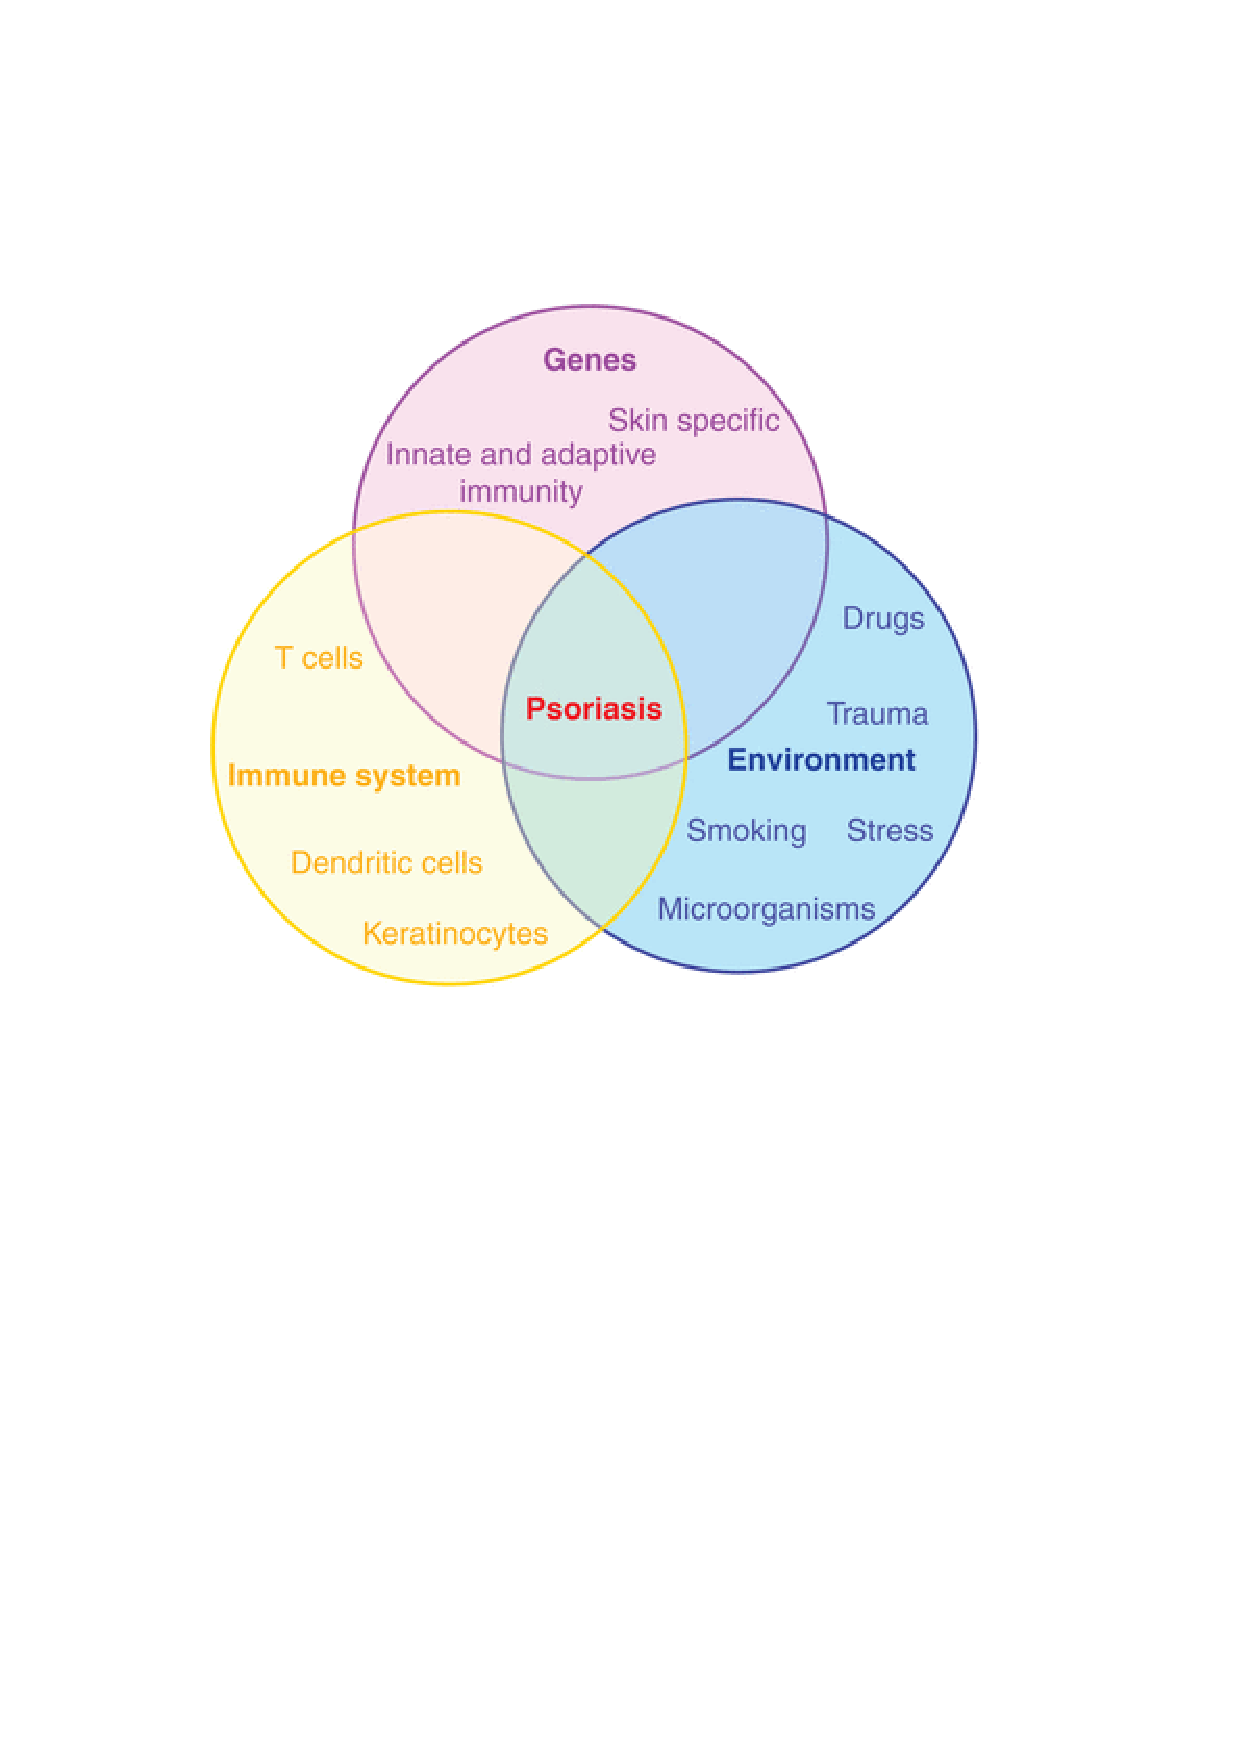
\includegraphics[width=\textwidth]{./Introduction/pdfs/PSO_aetiology_diagram_Di_Meglio_et_al_2014.pdf}
%\caption[Main factors involved in psoriasis disease aetiology]{\textbf{Figure adapted from \parencite{Meglio2014}}}
%\label{fig:PSO_aetiology_diagram}
%\end{figure}


\subsubsection*{Histopathological alterations in skin and joints}

The epidermis is the most external compartment of the skin, formed by approximately 90\% keratinocytes (KCs) and organised in a layer-like structure that self-renews in an spatial and time-dependent manner \parencite{Wikramanayake2014}. KC differentiation is associated with changes in morphology, replication ability and keratin composition of the intracellular matrix. In the context of psoriasis, impaired epidermis cell renewal leads to histological alterations and lesion development. Importantly, KCs undergo upregulation in the proliferation rate (hyperplasia) that causes aberrant cell differentiation (parakeratosis) thickening of the epidermis and the subsequent scale formation (Ruchusatsawat2011). Concomitantly, inflammation causes immune cell infiltration and hypervascularisation of the lesion driven by upregulation in the expression of angiogenic factors and activation of the endothelium \parencite{Perera2012}.  

In PsA, joint affection usually follows skin lesions and it involves a wide range of histological changes in the joints, particularly bone remodeling \parencite{Haddad2013}. One of the most common structural changes is the arthritis caused by the swelling and inflammation of the joints \parencite{Schett2011}. As result of this inflammation, alterations in bone remodeling leads to osteolysis with subsequent bone resorption and erosion at the affected joints \parencite{Mensah2017}. This phenomenon is particularly relevant in arthritis mutilans or chronic absortive arthritis, one of the most severe forms of PsA \parencite{Haddad2013}. Bone erosion is also the main histopathological process driving dactylatis, where bone lysis resolves in shortening of the digits \parencite{Gladman2005}. On the other hand, 35\% of the PsA patients undergo inflammation of the connective tissue at the insertion of tendons or ligaments, phenomenon known as enthesitis \parencite{McGonagle2011,Polachek2017}. Overtime, this causes debilitating structural changes due to formation of bony spurs along the insertion sites\parencite{Schett2011}.


\subsubsection*{Dysregulation of the innate and adaptive immune response}
%link to the histological changes
The dysregulated  immune response in psoriasis and PSA is the result of the interaction between innate and adaptive immune cells (ref section) resulting in feedback loops involving a complex cytokine milieu. Among the most relevant cytokines of the innate immunity involved in disease initiation are IFN-$\alpha$ and IFN-$\gamma$ \parencite{Leanne2009}. They are mainly produced by circulating plasmacytoid DC (pDC) and myeloid DC (mDC), respectively, upon activation by KC pro-inflammatory cytokines \parencite{Perera2012}. Both are upregulated at the mRNA level in the lesional skin and contribute to lymphocyte recruitment and maintenance of DC activation \parencite{Schmid1994}. 

Another key cytokine in this dysregulated inflammatory response is TNF-$\alpha$ which has a prominent role in bone turnover and bone remodeling in PsA \parencite{Mensah2008}. It is produced by activated KC, mast cells but also by adaptive immune cells types, including infiltrated T helper(Th) 1 and Th-17 cells infiltrated in the psoriatic lesion and PsA inflamed joints \parencite{Perera2012} and it induces activation of nuclear factor kappa-light-chain-enhancer of activated B cells (NF-$\kapa$B) signaling pathways (ref). It also activates several kinase signaling pathways as well as cell death programs (ref). In the context of inflammation, NF-$\kapa$B represents a master transcriptional regulator of both, the innate and adaptive immune system that induces expression of proinflammatory cytokines, antiapoptotic genes and genes involved in chronic inflammation maintenance (ref). The importance of this transcription factor (TF) in psoriasis and PsA pathogenesis is reflected by the association with disease of several genetic variants in some of the negative regulators of its proinflammatory activity, including NF-$\kapa$B inhibitor alpha \textit{NFKBIA} and TNF receptor-associated factor 3 interacting protein 2 \textit{TRAF3IP2} (ref).
 
Interleukin-23 (IL23) and Th17 axis represents a key loop for the maintenance of psoriasis and PsA inflammatory response and a very important link between innate and adaptive immunity. IL-23 is an innate regulatory cytokine, mainly produced by mDC and macrophages homing the inflamed skin and it binds to the IL-23 receptor (IL-23R), which expression is upregulated in the DC and T cells of the lesion and in circulating Th cells (ref). In psoriasis, IL-23 is the mediator for the pathogenic loop between activated KC and T cells (ref). Both IL-23 and IL-23R present protective and pathogenic genetic variants associated with psoriasis and PsA risk (ref). The activation of the IL-23 pathway leads importantly to increased IL-17 production through NF-\kappaB activation by \textit{TRAF3IP2} (ref). IL17 favors maintenance of the adaptive immune mediated Th17 response through recruitment and activation of neutrophils, induction of proinflammatory cytokines including IL-1\beta and IL-6 and also perpetuation of KC activation (ref) (https://www.ncbi.nlm.nih.gov/pmc/articles/PMC3580541/). % add info
More recently, interleukin 22 (IL-22) has arisen as another of the key cytokines in mediating the dysregulated cross talk between the innate and adaptive immune response. IL22 levels are increased in the psoriatic lesions and serum of patients and it is mainly produced by a subset of CD4$^+$ cells known as Th22 (ref). It mediates some of the histological changes in skin as well as AMP production by KC (ref).

% Maybe a paragraph to connect skin and joint affection Identical T cell clonality between skin and synovium https://ac.els-cdn.com/S0198885999000348/1-s2.0-S0198885999000348-main.pdf?_tid=5efa7316-fde5-11e7-8091-00000aacb360&acdnat=1516454913_dd20efb867f822d68d8b09873601e8ad

\subsubsection*{Environmental factors and disease}
Several environmental factors are known to be associated with increased risk and worsening of psoriasis and PsA development. A wide range of drugs including antidepressant, antihypertensive and anticytokine therapies have been clinically associated with initiation, exacerbation and worsening of psoriasis \parencite{Kim2010}. Infectious agents such streptococcal throat infection have also been associated with development of type I psoriasis \parencite{Gudjonsson2003,Valdimarsson2009, Diluvio2006}. Consistently with other chronic inflammatory disease such as IBD and AS, recent studies have also observed perturbation in the composition of the gut and skin microbiota in psoriasis and PsA patients \parencite{add reference}. Furthermore, physical trauma, including tattoos, surgical incisions and mechanical stress can trigger the appearance of skin lesions and digits joint inflammation \parencite {Weiss2002,Nestle2009}. Lastly, behavioral factors including smoking, alcohol and stress have been linked to psoriasis and PsA but no clear association with disease development has been established yet\parencite{Meglio2014}.

\subsection{Cell types involved in psoriasis and PsA pathogenesis}
%Global report on psoriasis, 2016

Psoriasis and PsA are complex dynamic pathophysiological processes, and the understanding of the relative importance of different cell types at different disease stages still remains challenging.

Several studies have shown the role of KCs as immune sentinels through MHC-II antigen presentation and production of antimicrobial peptides (AMP), cytokines and chemokines \parencite{Black2007}. Indeed, complex formation between the cationic AMP LL-37 and self-DNA/RNA released by KCs has been observed upon damage triggered by environmental factors \parencite{Lande2007}. This complex acts as an antigen for activation of the skin-resident DCs that initiate and perpetuate the skin inflammatory response through secretion of pro-inflammatory cytokines, including IL-1, IL-6 and TNF-$\alpha$ \parencite{Feldmeyer2007, Arend2008, Nestle2009, Nestle2005}. Furthermore, \textit{in vivo} studies have described the development of psoriatic lesions in immunodeficient mice upon human xenotransplant of psoriatic skin\parencite{Boyman2004}. Altogether, these findings support the role of epidermis dysfunction in the initiation of the psoriatic chronic inflammatory response \parencite{Proskch2008}.  The relevance of KCs at early stages of psoriasis pathogenesis is reinforced by the genetic association between KC-specific genes from the late cornified envelope (LCE) family and increased psoriasis risk \parencite{Tsoi2012}

mDCs and pDCs are also considered important innate immune cells in disease initiation through antigen presentation, T-cell activation and the subsequent adaptive immune response\parencite{Mahil20016}. pDCs are circulating professional antigen presentation cells (APCs) that only upon activation by the KCs self-DNA-LL-37 complex infiltrate into the lesional and uninvolved dermis of psoriasis patients \parencite{Nestle2005, Lande2007}. In contrast, quiescent mDCs are epidermal resident cells that undergo maturation in presence of the IFN-$\alpha$ secreted by pDCs, expanding up to 30-fold only in the lesional skin \parencite{Zaba2007}. The activated mDCs mediate the Th-1 and Th-17 response as well as perpetuation of KC activation through IL-23 production (ref). Studies in immunodeficient psoriasis mouse models have shown that blockage of downstream IFN-$\alpha$ signaling or IFN-$\alpha$ production by pDCs failed to induce T-cell activation and psoriasis onset \parencite{Nestle2005}. 


Neutrophils are also though to be closely involved in disease initiation through their ability to form neutrophil extracellular traps (NET)that contain host DNA and LL-37 \parencite{Hu2016}. There is evidence of increased NET formation in peripheral blood and lesional skin of psoriasis patients and they seem to be contributing to pDC and CD4$^+$ T activation \parencite{Hu2016}. Neutrophils have also been identified in recent studies as one of the main sources of IL-17 production in the skin lesions \parencite{Lin2011} and they also release a wide range of proteases which some induce KC proliferation \parencite{Mahil2006}.

In the context of the innate immunity, the involvement of monocytes and macrophages in psoriasis and PsA has not been extensively studied. Resident macrophages in the healthy dermis undergo a 3-fold increase upon skin lesion and they are involved in disease development through TNF$\alpha$ production \parencite{Perera2012, Mahil2016}. Similarly, mice models for chronic psoriasiform skin inflammation have shown macrophage migration into the affected skin and TNF-$\alpha$ production for maintenance of the skin lesions \parencite{Stratis2006, Wang2006}. Some studies using isolated monocytes from psoriasis patients PBMC  have shown greater phagocytic and bactericidal activity compare to those from healthy individuals \parencite{Bar-Eli1979}. Later studies have also shown increased circulating intermediate monocytes (CD14$^{+}$ high CD16$^{+}$ high) and monocyte aggregation in psoriasis patients causing enhanced platelet activation and angiogenesis \parencite {Golden2015}. In PsA, synovial membranes levels of monocytes/macrophage metalloproteinases which mediate bone erosion through differentiation into osteoclasts are comparable to those found in RA joints \parencite{Hitchon2002}. Overall, these observations highlight the systemic aspects of both pathologies. 

%HLA-Cw*06:02 can be recognised by the inhibitory receptor KIR2DL1 and the activatory receptor KIR2DS1.  Some studies have shown KIR2DS1 was present in 85\% of the patients but only in 51\% of the controls
%NK cells are important regulators of immune responses \parencite{Luszczek2004}. Their function extends beyond killing of infected or transformed cells. Interactions with dendritic cells, macrophages, and fetal trophoblast cells can regulate NK cell activity by influencing cytokine production, cytotoxicity and stimulation of T helper-1 responses. 
%
%


In the context of the innate immunity, the involvement of monocytes and macrophages in psoriasis and PsA has not been extensively explored. Resident macrophages in the healthy dermis undergo a 3-fold increase upon skin lesion and contribute to disease development through TNF$\alpha$ production \parencite{Perera2012, Mahil2016}. Similarly, mouse models for chronic psoriasiform skin inflammation have shown the role of macrophage migration into the affected skin and production of TNF-$\alpha$ in maintenance of the skin lesions \parencite{Stratis2006, Wang2006}. Initial studies showed greater phagocytic and bactericidal activity of PBMCs isolated monocytes from psoriasis patients compared to those from healthy individuals \parencite{Bar-Eli1979}. Additionally, increased circulating intermediate monocytes (CD14$^+$ high CD16$^+$ high) and monocyte aggregation was also observed in psoriasis patients, resulting in enhanced platelet activation and angiogenesis \parencite {Golden2015}. In PsA synovial membranes, the levels of monocytes/macrophage metalloproteinases responsible for bone erosion through differentiation into osteoclasts  have been found to be similar to those  found in rheumatoid arthritis (RA) joints \parencite{Hitchon2002}. 

Regarding the adaptive immunity, T lymphocytes have been considered the most relevant cell types in the initiation and maintenance of psoriasis and PsA. Report cases in humans have demonstrated that bone marrow transplantation can initiate or terminate psoriasis \parencite{Eedy1990, Gardembas1990}. Reduced numbers of circulating T cells but increased percentages of the memory populations CD4$^+$CD45RO$^+$ and CD8$^+$CD45RO$^+$ have been observed in moderate-to-severe and severe psoriasis patients when compared to milder phenotypes and healthy controls \parencite{Lecewicz-Toruń2001,Langewouters2008}. Different studies have reported controversial results regarding the total abundance and ratios of CD4$^+$ and CD8$^{+}$ in PBMC, likely due to the phenotype heterogeneity of the psoriasis cohorts between studies \parencite{Lecewicz-Toruń2001,Cameron2003,Langewouters2008}. In PsA, no differences in abundance of circulating T cells have been identified when compared to healthy individuals \parencite{Costello1999}.

In homeostasis, CD8$^+$ and CD4$^+$ lymphocytes are found in the epidermis and dermis, respectively \parencite{Clark2006}. An increase in activated memory CD4$^{+}$CD45RO$^{+}$and CD8$^{+}$CD45RO$^{+}$ cells can be detected by the third day from the lesion appearance \parencite{Clark2006,Perera2012 }. \textit{In vivo} studies showed that development of psoriasis following engrafted human pre-lesional skin was only dependent on local T cell proliferation, highlighting the importance of circulating T cells recruitment during the priming event rather than at later stages of the disease \parencite{ Boyle2013,Perera2012}. The relative importance of CD4$^+$versus CD8$^+$ cells in psoriasis initiation has been explored in pre-lesional skin mouse xenografts where CD4$^+$ but not CD8$^+$ T cells were required in the transition from uninvolved to lesional skin \parencite{Nickoloff1999}. Interestingly, the injection of activated CD4$^+$ cells in mice was followed by an acute increase in activated resident CD8$^+$ T cells. Overall, these results supported the hypothesis of skin CD4$^+$ cells being drivers of resident T-cell activation and the population of resident activated CD8$^+$ the main effector of the immune response. In synovial tissues of PsA patients, CD4$^+$ are significantly more abundant than CD8$^+$ \parencite{Diani2015}. However, amongst the CD8$^+$ populations, the memory cells are prevalent in the patients’ synovial fluid (SF) with a significant enrichment compared to controls \parencite{Costello1999}. The contribution of regulatory T (Treg) remains controversial in both, psoriasis and PsA \parencite{Perera2012}. 

Based on the cytokine profile, psoriasis and PsA have been classified as a type 1 Th/Tc disease, where activation of naive CD4$^+$ and CD8$^+$ cells is driven by IL-12 and IFN-$\gamma$ \parencite{Austin1999,Perera2012}. In addition, T-cell subsets including Th-17/Tc-17 and Th-22/Tc-22, producing high levels of IL-17 and IL-22, respectively, have been identified to be relevant for the perpetuation of the inflammatory response \parencite{Mahil2016}. The importance of Th-17 cells and IL-17 production has been evaluated in skin, joints and blood, with elevated mRNA and protein levels of IL-17 and also IL-23 reported in psoriasis and PsA patients compared to controls \parencite{Cai2012, Dolcino2015}. The relevance of IL-17 has been further highlighted by the presence of CD8$^+$ populations in patients’ SF that are predominantly IL-17 producers and whose abundance correlates with markers of inflammation and structural changes in the joint \parencite{Menon2014}. This finding is in line with observations in skin and suggests a prominent role for CD8$^+$ IL-17-producing cells in the different stages of both pathologies. Studies directed to understand the importance of IL-17 have led to the discovery of other immune cells producing this pivotal cytokine, including innate immune lymphoid (ILC) cells and $\gamma$$\delta$ T cells, opening new research avenues in the context of psoriasis and PsA pathophysiology and treatment \parencite{Meglio2014,Leijten2015}. IL-17-producing cells have also been hypothesised to be at the link between skin and joint lesions. Although the precise mechanisms for transition between psoriasis and PsA is still poorly understood, the study of psoriasis and RA in mouse models revealed that skin lesions facilitate arthritis and joint inflammation \parencite{}. %In fact, the presence of IL-17-producing cells in the inflamed skin nearby the enthesis of joints under physical stress is likely to be a trigger for the development of PsA.

\begin{figure}[H]
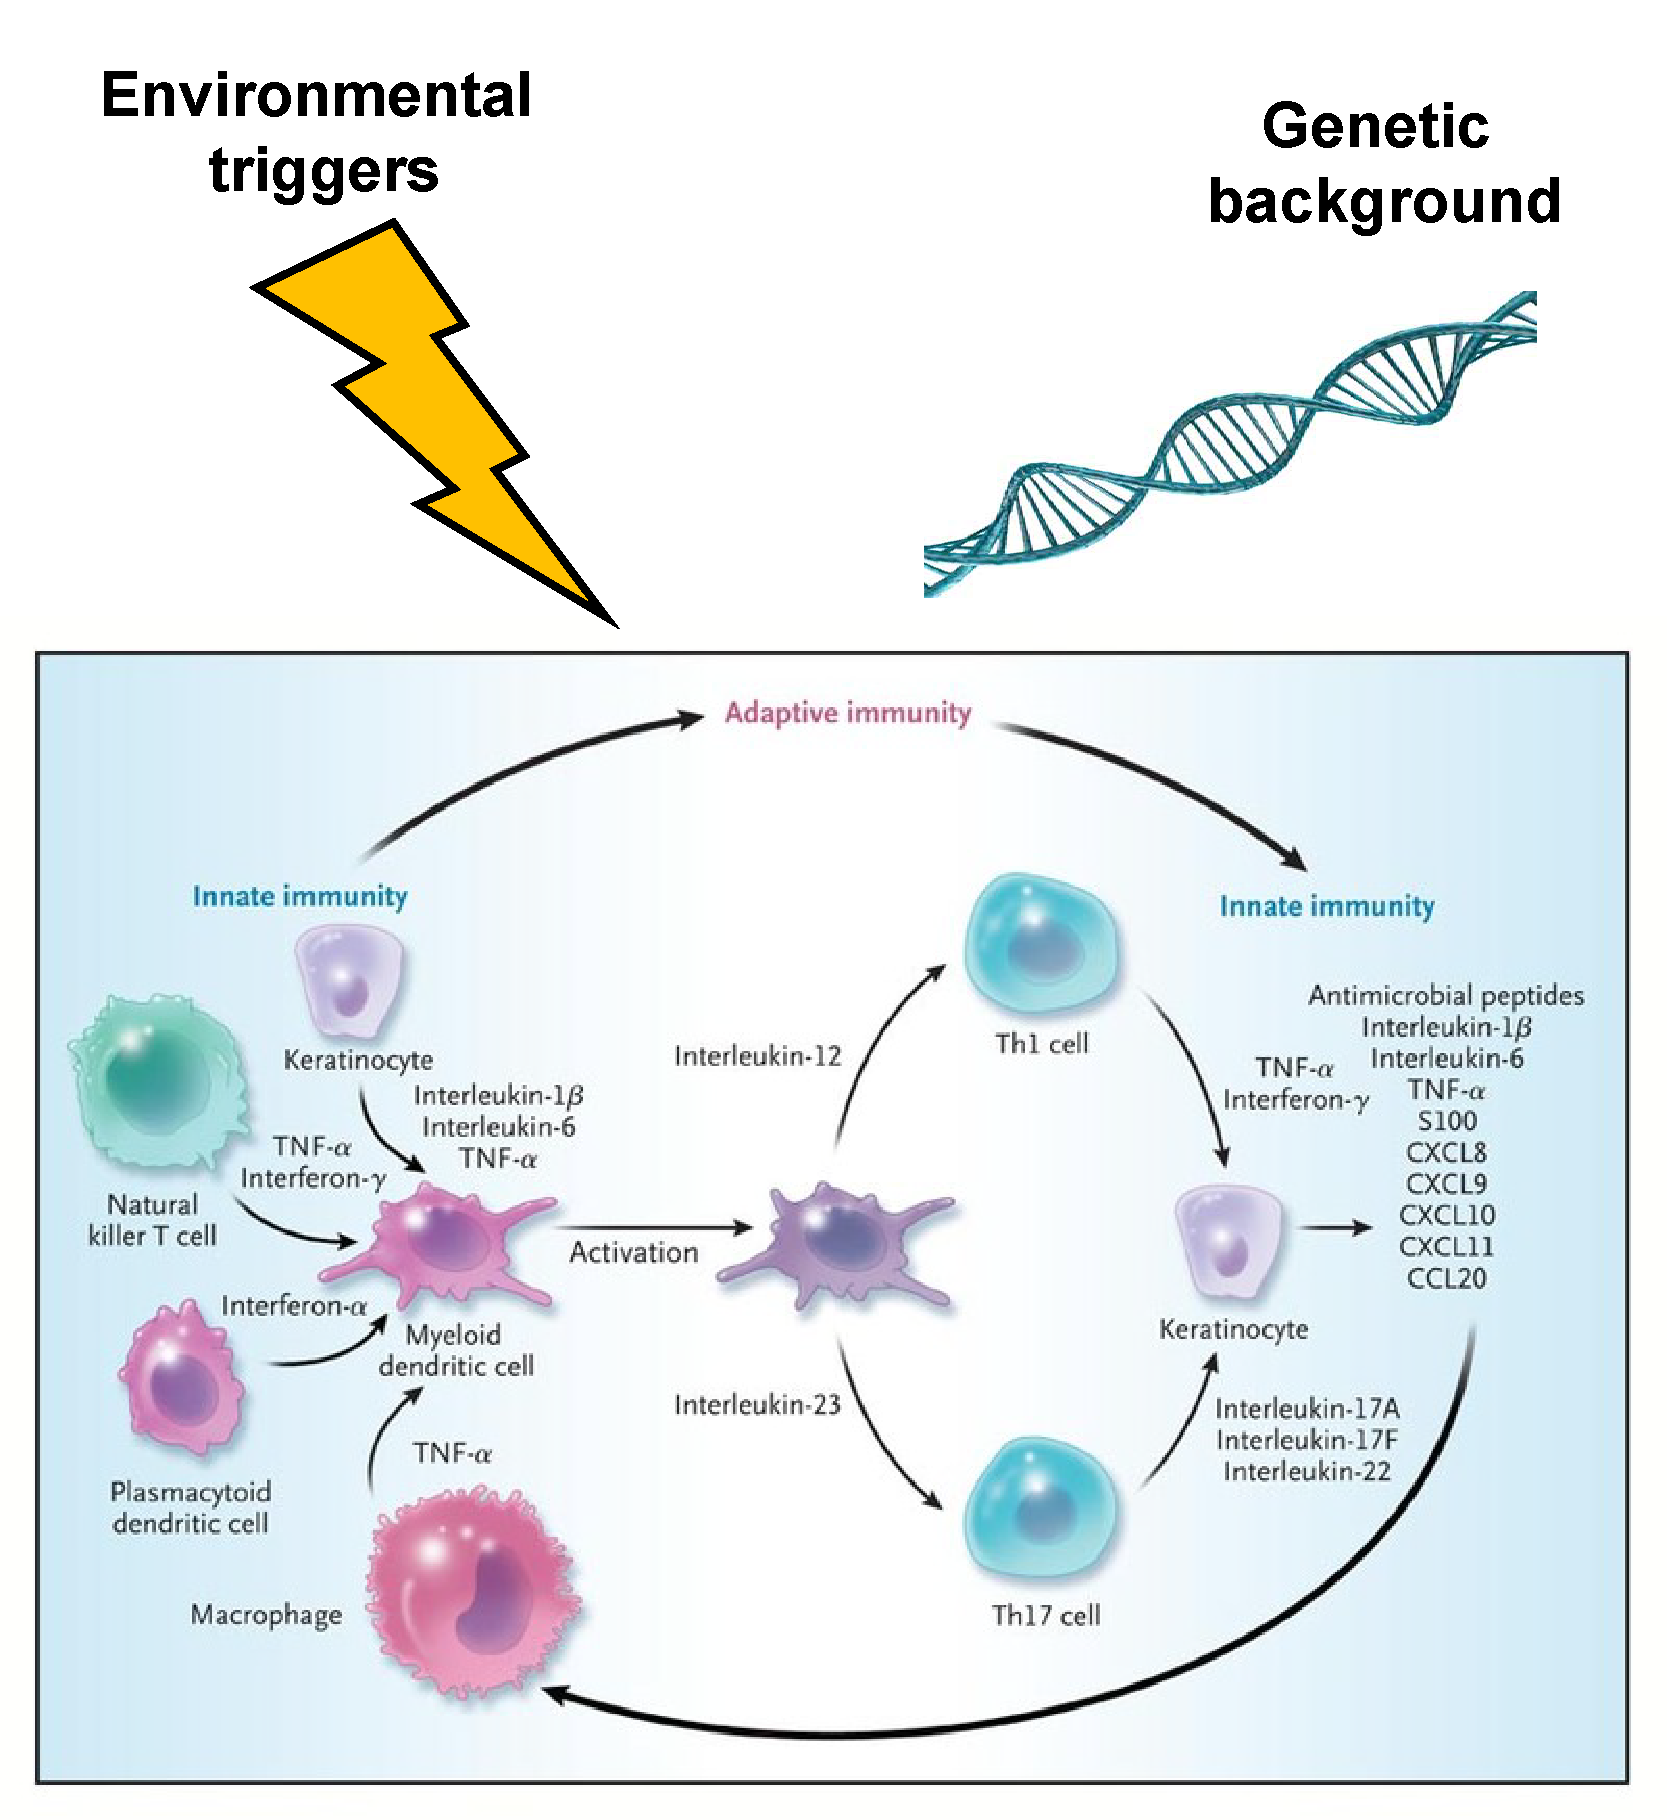
\includegraphics[width=\textwidth]{./Introduction/pdfs/PSO_adaptive_innate_immune_system_crosstalk.pdf}
\caption[Crosstalk between innate and adaptive immunity in psoriasis]{\textbf{Figure adapted from \parencite{Nestle2009}}}
\label{fig:PSO_immune_system_diagram}
\end{figure}

\subsection{Therapeutic intervention}
Nowadays, psoriasis or PsA are still incurable diseases and the different treatments available are solely focused in alleviating the symptoms. For instance, topical therapies are the choice in cases of mild-to-moderate psoriasis, represented by the extended emollients and short-term corticosteroids, due to associated side-effects \parencite{Menter2009}. In psoriasis, other topical treatments are used in combination with corticosteroids such ultraviolet (UV) light therapy and vitamin D analogues, directed to inhibit T-cell and KC proliferation, and stimulate KC differentiation \parencite{Rizova2001}. In the case of PsA patients presenting swelling of two or less joints, intra-articular injection of glucocorticosteroids together with joint aspiration is used as a short-term solution to reduce pain and inflammation \parencite{Coates2016}. Nonetheless, treatment of most forms of PsA and moderate-to-severe psoriasis require the use of systemic therapies. Patients presenting mild cases of PsA commonly receive nonsteroidal anti-inflammatory drug (NSAID) to control the inflammatory symptoms \parencite{Coates2016}. More severe forms of PsA require the use of disease-modifying antirheumatic drugs (DMARDs) including the antagonist of folic acid methotrexate (MTX) and the phosphodiesterase 4 inhibitor Apremilast that act as immunosuppressors of activated T cells and cytokine production, respectively \parencite{Schmitt2014, Gossec2016, Keating2017,Polachek2017}.
Remarkably, biologic systemic agents represent the most specific treatment option for severe psoriasis and PsA. This category encompasses an array of cell-based molecular species that modulate the immune response in a physiological manner \parencite{Perera2012}. Specifically, the relevance of TNF-alpha in psoriasis and PsA has led to the extensive therapeutic use of TNF-alpha inhibitors during the past five decades, making them the ‘drugs of choice’ amongst all the biologic agents targeting cytokine pathways. Three TNFi have been approved for the treatment of psoriasis: etanercept, infliximab and adalimumab \parencite{Ahil2016}. In addition to those, certolizumab pegol and golimumab are often applied in the management of PsA and other rheumatoid diseases \parencite{Coates2016b}. Although TNF-$\alpha$ blockade is one of the most effective treatments, side effects such as increased risk of infection, or reactivation of latent infections have been identified \parencite{Nickoloff2004}. Moreover, between 20 to 50\% of the patients fail to respond to the first TNFi administrated, requiring switching to alternative TNFi \parencite{Abramson2016}. New biologic therapies have been developed to target other key cytokines in the pathogenesis of PsA and psoriasis, such as IL-12, IL-23 (ustekinumab) or IL-17 (secukinumab and ixekizumab) and represent a substantial benefit for treating patients failing to respond to TNFi \parencite{Mahil2016, Coates2016b}.

% Bispecific antibodies
 

\section{Genetics of psoriasis and psoriatic arthritis}

As complex diseases, the risk to develop psoriasis and PsA is not only influenced by the surrounding environmental conditions but also by the genetic background of each individual. Determining the magnitude of contribution of the genetic factors in the development of these diseases and identifying the exact genes or genomic regions involved in the predisposition to psoriasis and PsA remains challenging.  


\subsection{Heritability}

Several studies have shown a trend towrads the increase of psoriasis and PsA prevalence over the last 30 years in different countries \parencite{Organization2016}. This importantly reflects changes in life style habits and it highlights the need to better understand the genetic factors that predispose to disease upon interaction with environmental stresses.

The contribution of genetics in the development of psoriasis has also been demonstrated in several twins studies. The concordance of psoriasis has been shown to be greater in monozygotic (33-55\%) compared to dizyogtic (13-21\%), estimating an 80\% of heritability in this condition \parencite{Faber1974, Duffy1993, Pendersen2008}. Conversely, similar concordance between mono- and di- zygotic twins has been reported in the case of PsA, probably due to lack of statistical power and appropriate diagnosis \parencite{Pendersen2008}. In the general population, approximately 40\% of the patients with psoriasis or PsA have family history in first degree relatives \parencite{Gladman1986}. Interestingly, the recurrence in first-degree relatives has been shown to be greater in PsA (40) compared to psoriasis (8) in a study in Icelandic population \parencite{Chandran2009}. This suggests differences in the heritability between the two phenotypes and a stronger genetic contribution in PsA.

\subsection{Non-GWAS and linkage studies}
Different approaches have been undertaken to uncover the genetic variability predisposing to psoriasis and PsA. The appearance of next generation sequencing (NGS) techniques and the progressive reduction of cost has allowed to move from single locus gene candidate studies to a genome-wide approach.
The study of psoriasis and PsA genetic architecture started with linkage analyses in family pedigrees presenting an autosomal dominant condition. This approach yielded nine psoriasis susceptibility loci (PSORS1-9) with PSORS1 showing the strongest genetic association \parencite{Capon2017, International2003}. The PSORS1 locus lies within the MHC I region in chromosome 6p21, previously associated with psoriasis susceptibility in serological studies \parencite{Rusell1972, Tiilikainen1980}. Importantly, Mendelian forms of disease with rare highly penetrant mutations have also been identified in family studies for two genes within PSORS2 (17q25): zinc finger protein 750 (\textit{ZNF750}) and caspase domain family member 14 (\textit{CARD14}) \parencite{Tomfohrde1994,Jordan2012}. Rare gain of function and \textit{de novo} mutations and also common variants in \textit{CARD14} have been identified in psoriasis and PsA patients, suggesting an important role of the genetic variation in this gene for Mendelian and multi-factorial forms of disease \parencite {Jordan2012, Tsoi2012}. %In PsA, a region close to the psoriasis PSORS8 was also identified \parencite{Karason2003}. 
Nevertheless, the inability of independent studies to reproduce the results for regions other than PSOR1, 2 and 4, highlighted the limitations of the linkage studies to understand the genetics of complex diseases \parencite{Capon2017}. Additionally, gene based studies in psoriasis and PsA disclosed the importance of genetic variability in the activating killer immunoglobulin receptors 2DS1 (\textit{KIR2DS1}) gene, also reported for AS and RA, which interestingly is mainly triggered by interaction with HLA-Cw*06:02 \parencite{Łuszczek2004, Williams2005,Carter2007, Yen2001}.  

%Similarly, specific association with PsA but not psoriasis was found for microsatellites and promoter polymorphisms in TNF-$\alpha$ \parencite{H\"{o}hler2002}. 

\subsection{Genome-wide association studies}

The dramatic advances in sequencing and genotyping technologies have allowed the implementation of association studies at a genome-wide scale. The genome-wide association studies (GWAS) have benefitted from the understanding of common single base-pair changes know as single nucleotide polymorphisms (SNPs) in different populations through whole genome sequencing (WGS) projects such as HapMap \parencite{The international HapMaP Consortium} and the 1000 Genomes \parencite{The 1000 Genomes}. GWAS generally focus in identifying disease-associated common SNPs (with minor allele frequency (MAF) ${>}$5\% ) showing with differences in allele frequency between patients and controls \parencite{Ku2010}. GWAS design are thus based on the hypothesis that complex diseases are more likely to be caused by the interaction of multiple common variants, showing greater power than the previous linkage studies to identify multiple loci with low penetrance and moderate to small effects \parencite{Schork2009, Cui2010}. 

Due to the organisation of the genome into segments of strong linkage disequilibrium (LD) where genetic variants are strongly correlated with each other, the genotyped SNPs in GWAS are solely used a proxy for the disease causative variant. Therefore, disease causal variants can be non-genotyped SNPs or other type of genetic variability such as copy number variants (CNVs), also highly frequent in the genome but less widely studied by GWAS \parencite{Hirschhorn2005, Ku2010}. 

Since 2007, when the first psoriasis and PsA GWAS were published, a total of sixty-three genetic associations have been identified at a genome-wide significance (pval>5x10$^-8$) which explain 28\% of the psoriasis and PsA heritability (Table \ref{tab:GWAS_studies}) \parencite{Tsoi2017}. The majority of the studies have been performed in Caucasian European or North American cohorts but more recently, GWAS studies in Chinese populations have also been published \parencite{Zhang2009, Sun2010, Yin2015}. Initial studies were performed in discrete cohort sizes with moderate power that confirmed association with loci overlapping the PSOR1, PSOR2 and PSOR4 genomic regions from the linkage studies \parencite{Strange2010}. Specifically, HLA-C has been consistently identified as the most significant locus with the greatest effect size. Additional MHC-I and MHC-II associations with disease risk have been identified for HLA-A, HLA-B and HLA-DQA1 through step-wise conditional analysis\parencite{Okada2014}. The information extracted from GWAS studies was significantly enhanced with the use of the Immunochip genotyping platform, which covers 186 immune relevant loci identified in previous GWAS studies across different inflammatory diseases at a greater genotyping density \parencite{Tsoi2012}. The psoriasis Immunochip study uncovered fifteen new associations and also included meta-analysis with the largest available psoriasis cohorts at the time\parencite{Tsoi2012}. This meta-analysis has been expanded further, with sixteen additional associations in the latest study reinforcing the importance of NF$\kappa$B and cytotoxicity pathways in disease pathophysiology \parencite{Tsoi2015,Tsoi2017}.

Meta-analysis of GWAS across Caucasian and Chinese populations have showed the value of this trans-ethnic approach to identify new associations and understand the differences in the genetic associations contributing to disease risk in different populations \parencite{Yin2015}. %Four new non-coding loci in the vicinity of \textit{LOC144817}, \textit{COG6}, \textit{RUNX1} and \textit{TP63} were associated with psoriasis and PsA in both populations. Interestingly, genetic heterogeneity between Caucasian and Chinese cohorts was also observed for ten of the GWAS reported loci, for example \textit{ELMO1} and \textit{TYK2}.
In addition to discrepancies in first degree relatives heritability, changes in the frequencies of HLA-C and HLA-B alleles had also evidenced genetic differences between psoriasis and PsA, supporting the importance of conducting independent GWAS studies \parencite{Winchester2012, Okada2014}. In fact, cohort stratification confirmed specific association with PsA for previously identified psoriasis loci such as \textit{TRAF3IP}, \textit{IFNLR1}, \textit{IFIH1} and \textit{NFKBIA} and PsA-specific independent signals for \textit{IL23R} and \textit{TNFAIP3} \parencite{Ellinghaus2010, Stuart2015}.  Interestingly, the association for \textit{LCE3C/B},identified in combined phenotypic studies, showed greater strength in those psoriasis patients affected for over ten years without developing joint affection \parencite{Stuart2015}. Lately, PsA GWAS using the Immunochip platform revealed a PsA-specific association in chromosome 5q31 \parencite{Bowes2015}. 

Altogether, GWAS studies have demonstrated shared genetic susceptibility between psoriasis and PsA, but have also highlighted intrinsic specificity that may support a difference in the genetic architecture of both diseases. It is important to take into account that these results are affected by imprecise phenotyping of cases, which entails one of the many challenges in the comparison of both diseases.


%
\begin{landscape}
\begin{center}
\begin{longtable}[ht]{c c c c c}
%{p{.15\textheight} p{.15\textheight} p{.25\textheight} p{.25\textheight} p{.15\textheight} p{.15\textheight} p{.15\textheight}}
\caption[Main GWAS studies in psoriasis and PsA]{\textbf{Main GWAS studies in psoriasis and PsA.} Summary table describing the most relevant psoriasis and PsA GWAS studies. Information regarding sample size, patients phenotypes and the main reported associations in each study is included. The Ellinghaus \textit{et al.}, 2010 and the Stuart \textit{et al.}, 2015 studies included stratified association analysis of psoriasis and PsA independently. $^\star$ Meta-analysis performed.}
\label{tab:GWAS_summary} \\
\toprule
\textbf{Study} & \textbf{Etnicity} & \textbf{Sample size}      & \textbf{Phenotype} & \textbf{Main associations} \\
               &                   & \textbf{(Cases/Controls)} &                    &  \textit{(putative genes)}                  \\
\midrule
\midrule
\parencite{Cargill2007} &	White North American &	1,446/1,432 &	Psoriasis and PsA &	HLA-C (PSOR1) and \textit{IL12B} \\
\parencite{Nair2009} &	European	& 1,409/1,436 &	Psoriasis and PsA &	\textit{IL23A}, \textit{IL23R}, \textit{IL12B}, \textit{TNIP1}, \textit{TNFIP3}, \textit{IL4} and \textit{IL13} \\
\parencite{Stuart2010} &	White North American and European &	1,831/2,546	& Psoriasis and PsA &	\textit{NOS2}, \textit{FBXL19},\textit{PSMA6-NFKBIA} \\

\parencite{Ellinghaus2010} &	German	& 472/1,146	& Psoriasis	& \textit{TRAF3IP2} \\

\parencite{Strange2010} &	European & 2,622/5,667 & Psoriasis and PsA & \textit{LCE3D} (PSOR2), \textit{IL28RA}, \textit{REL}, \textit{IFIH1}, \textit{ERAP1}, \textit{TYK2} and \textit{HLA-C/ERAP1} epistasia \\

\parencite{Zhang2008} & Chinese	& 1,139/1,132	& Psoriasis type I & \textit{LCE} gene family and \textit{IL12B} \\

\parencite{Sun2010} & Chinese	& 8,312/12,919	& Psoriasis and PsA &	\textit{ERAP1}, \textit{PTTG1}, \textit{CSMD1}, \textit{GJB2}, \textit{SERPINB8} , \textit{ZNF816A} \\

\parencite{Tsoi2012}$^\star$ & White North American and European & 10,588/22,806 & Psoriasis and PsA & \textit{CARD14} (PSOR4), \textit{RUNX3}, \textit{B3GNT2}, \textit{ELMO1}, \textit{STAT3} \\

\parencite{Tsoi2015}$^\star$	& White North American and European	& 15,000/27,000	& Psoriasis and PsA	& 1q31.1, 5p13.1, \textit{PLCL2}, \textit{NFKBIZ}, \textit{CAMK2G} \\

\parencite{Bowes2015} &	British, Irish and Australians	& 1,962/8,923	& PsA	& 5q31 PsA-specific \\

\parencite{Stuart2015} &	White North American and European	& 1,430/1,417	& Psoriasis and PsA	& \\

\parencite{Tsoi2017}$^\star$ &	White North American and European	& 19,032/39,498	& Psoriasis and PsA	& \textit{CHUK}, \textit{IKBKE}, \textit{FASLG}, \textit{KLRK1}, \textit{PTEN} \\																		
\bottomrule
\medskip
\end{longtable}
\end{center}
\end{landscape}



\subsection{Relevance of non-coding versus coding variants in disease susceptibility}

Approximately 88\% of all GWAS associations map within non-coding regions and only the remaining 12\% account for coding variants likely to cause non-synonymous mutations impacting in the protein function \parencite{Welter2013}.

%-Coding variants are an small proportion: e.g in psoriasis and PsA from exome wide studies. Say that associations could come through LD of coding variants but not always. Examples in psoriasis
Exome psoriasis association studies in Chinese and Caucasian populations have increased the number of coding variants with putative effect in the protein structure \parencite{Tang2014,Zuo2015,Dand2017}. These studies have confirmed some of the previously identified missense associations in \textit{CARD14} or \textit{ERAP1}, revealed new common coding variants at previously associated loci and identified protective rare missense changes, for example in the \textit{TYK2} gene\parencite{Tang2014,Dand2017}. Nevertheless, results from extensive exome studies suggest that non-synonymous SNPs have a limited contribution to the overall genetic risk of psoriasis compared to non-coding variants \parencite{Tang2014}.

The association of non-coding variants with disease can be explained by their ability to regulate gene expression in a cell and context specific manner \parencite{Fairfax2012}. These variants can be located at different regulatory elements, including enhancer, silencers, promoters and the 5' and 3' untranslated region (UTR) of genes \parencite{Ward2012}. Non-coding GWAS variants can alter the expression of target genes through different mechanisms including changes in chromatin accessibility, histone modifications, protein binding such as transcription factors, DNA methylation and binding of non-coding  RNA molecules\parencite{Knight2014} (Section 1.4.X).

Identification of the target gene regulated by non-coding variants represents a challenge in the field of functional genetics. This can be partially addressed by conducting expression quantitative trait loci (eQTL) analysis, which identifies genome-wide statistical associations between gene transcript levels and SNPs in \textit{cis} ($<$1Mb) or \textit{trans} to the gene. In T2D such approach revealed a \textit{cis}-eQTL for expression of the TF \textit{KLF4} and a haplotype of non-coding GWAS SNPs located 14Kb up-stream \parencite{Small2011}. Moreover, this haplotype also showed association with genes in \textit{trans}, highlighting downstream targets regulated by KLF4. Nevertheless, eQTL mapping alone only provides instances for transcriptomic regulation and additional functional assays, such as chromatin conformation, are required to demonstrate causality \parencite{Edwards2013}.  


\subsection{The role of GWAS studies in highlighting immune-relevant cell types and pathways}

GWAS represent a biologically unbiased approach to shed some light into pathophysiological relevant cell types and molecular pathways associated with disease. In the field of common immune-mediated diseases, GWAS have underscored some of the most important cell types for which genetic variation is functionally relevant. For example, in T2D the strongest GWAS associations showed to be enriched at pancreatic $\beta$ cells and to affect genes involved in insulin secretion, consistently with the insulin resistance that characterises the disease pathology \parencite{Visscher2017}.

Immune diseases have benefited from the use of the immune targeted genotyping array Immunochip to perform a systematic comparison of the genetic architecture across the different conditions. For example psoriasis and PsA share risk loci with AS, CD, MS, RA and T1D, among others \parencite{ImmunoBase}. However, genetic overlap where the signal is the same across different diseases have not necessarily the same direction and a risk allele for one can be protective for another reflecting true differences in the pathophysiology of different immune mediated diseases. The better understanding of immune-related diseases has led to identification of shared susceptibility loci and the use of therapeutic interventions across diseases, such as anti IL-23 and anti IL-17 antibodies to treat psoriasis, PsA, AS and IBD \parencite{Visscher2017}.Cross disease association studies have also been performed for the simultaneous analysis of AS, UC, primary sclerosing cholangilitis (PSO), CD and psoriasis \parencite{Ellinghaus2016}. This study revealed the greatest genetic pleiotropy of psoriasis with AS and CD, this meaning same alleles predisposing to disease risk \parencite{ImmunoBase}. Among the 206 multi-trait associated loci, enrichment was found for regulatory elements in bone marrow, NK and T cells as well as for immune response pathways, supporting the contribution of GWAS to the biological understanding of disease. In the case of psoriasis and PsA, most of the GWAS risk loci highlight genes that belong to a small number of pathways and they are enriched for regulatory elements of several cell types \parencite{Capon2017}. Nevertheless, it is important to bear in mind that in most of the cases non-coding variants from GWAS studies lack of functional characterisation and they tend to be associated arbitrarily to the nearest gene or the closest gene which fits into current knowledge about pathophysiology. This bias to some extent the genes that contribute to enrichment of certain pathways and the efficacy of drugs developed to target some of those genes has helped to further confirm their truly involvement in disease.

\subsubsection*{Antigen presentation}
\textit{HLA-Cw*0602}, the strongest GWAS association in psoriasis is also associated with other diseases such as Hepatitis C, PSO and Grave´s disease \parencite{Blais2011}. \textit{HLA-Cw*0602} is involved in antigen presentation and the absence of differences at the transcript level between normal and psoriatic individuals suggests the association is not explained by alteration in regulation of gene expression \parencite{Hundhausen2012}. The relevance of antigen presentation in psoriasis and PsA has been reinforced by the GWAS association of the endoplasmic reticulum aminopeptidase 1 \textit{ERAP-1} gene, which codes for an aminopeptidase involved in the trimming of peptide antigens. GWAS studies identified that \textit{ERAP-1} was associated with psoriasis and PsA only in individuals carrying one copy of the rs10484554 \textit{HLA-C} risk allele \parencite{Strange2010}. Moreover, the same studied also found dependent association of an SNP nearby the zeta chain of T cell receptor associated protein kinase 70 \textit{ZAP70} gene and \textit{HLA-Cw*0602}. ZAP70 is a tyrosin kinase that binds the CD3-$\zeta$ of the TCR and it is involved in the CD8$^+$ cells auto-reactivity regulation \parencite{Picard2009}, overall highlighting the role of HLA-dependent CD8$^+$ dysregulation in psoriasis and PsA. At the clinical level, \textit{HLA-Cw*0602} and \textit{ERAP-1} have also been associated with pediatric psoriasis onset together with other GWAS loci \parencite{Bergboer2012}. These epistatics phenomena, where association of one gene is dependent by the presence of another, has also been found between other HLA class I molecules such as \textit{HLA-B*27} and \textit{HLA-B40} and \textit{ERAP1} in AS \parencite{Evans2011, Cortes2015b}. The signal at chromosome 5q15 for \textit{ERAP1} allele is the same in psoriasis and AS and they also share the direction of the effect \parencite{ImmunoBase}. Several studies have revealed that the disease associated polymorphisms in AS increased \textit{ERAP-1} and \textit{ERAP-2} gene expression and also altered splicing, resulting in ERAP-1 protein isoforms with increased activity \parencite{Constatino2015, Hanson2018}.
Regarding cell types, the role DC and macrophages involved in antigen presentation is reinforced by genetic evidence.
%ERAP2 association with Romanian population in PsA in Romanian population https://link.springer.com/content/pdf/10.1007/s00005-016-0444-4.pdf 

%Only a small number of these genomic segments span a single gene, with the majority encompassing multiple transcripts and some mapping to gene deserts. Capon 2017

\subsubsection*{Skin barrier}
GWAS have highlighted KC specific genes such the \textit{LCE} gene cluster or genes with a very relevant role in the skin such as \textit{CARD-14}, both previously mentioned. Further studies in the \textit{PSORS4} have revealed that association with diseases is due to a deletion comprising two of the genes within this family, \textit{LCE3B} and \textit{LCE3C} (\textit{LCE3C\textunderscore LCE3B\textunderscore del})\parencite{Cid2009}. In normal skin, expression of \textit{LCE3B} and \textit{LCE3C} is very low and it is induced upon barrier disruption. These are proteins that form the cornified envelope on the most external layer of the epidermis and are thought to be involved in epidermal terminal differentiation \parencite{Bergboer2011}. Additionally, epistasia between this deletion and \textit{HLA-Cw*0602} has been identified in certain populations including Dutch and American \parencite{Cid2009, Riveira-Munoz2011}. Overall, the lack of \textit{LCE3B} and \textit{LCE3C} expression in psoriasis patient could lead to an impaired repair following skin disruption and facilitate microorganisms infection and the triggering of the dysregulated immune response. Treatment of psoriasis patients with UBV radiation have proved upregulation of \textit{LCE3E} expression after 48 hours contributing to amelioration of the skin lesions\parencite{Jackson2005}. \textit{CARD14} is primarily expressed in epithelial tissues where it is involved in recruitment and activation of the NF-$\kappa$B pathway \parencite{Blonska2011}. Common and rare pathogenic mutations of \textit{CARD14} in KC cell lines led to increased activation of NF-kB as well as overexpression of psoriasis-associated genes including \tetxit{IL6}, \textit{IL36}, \textit{TNFA} and \textit{TNFAIP2}, among others \parencite{Jordan2012b}.
%https://www.sciencedirect.com/science/article/pii/S0002929712001577?via%3Dihub


\subsubsection*{NF-$\kappa$B and TNF pathways}

The NF-$\kappa$B pathway is involved in the regulation of the innate and adaptive immune response. Several psoriasis and PsA GWAS loci have been mapped to gene members of the NF-$\kappa$B and TNF signaling pathway such as \textit{TNIP1}, \textit{TNFAIP3}, \textit{NFKBIA}, \textit{REL}, \textit{TRAF3IP2}, among others %refernce the GWAS table
\textit{NF-$\kappa$B} is a dimeric TF, formed by assembly of two of the five proteins from the NF-$\kappa$B family, that translocates into the nuclei upon cytokine stimuli, importantly TNF-$\alpha$. Dysregulation of a feedback loop between TNF-$\alpha$ and NF-$\kappa$B contributes to the development of many chronic inflammatory diseases \parencite{Liu2017} and neutralisation of TNF-$\alpha$ is used for treatment of many immune-mediated diseases, as previously described. In psoriasis, elevated levels of NF-$\kappa$B are found in lesional skin compared to uninvolved and normal skin \parencite{Lizzul2005}. Psoriasis and PsA GWAS association with \textit{NFKBIA}and \textit{REL}, two of the genes coding for \textit{NF-$\kappa$B} subunits, are driven by SNPs at an intergenic region, not having yet directly evidence to their effect over regulation of these genes \parencite{GWAS studies}. \textit{REL} has been associated with other inflammatory diseases, including CD and RA \parencite{ImmunoBase} and, interestingly, the RA risk allele has a protective effect in PsA showing opposite direction effects \parencite{Bowes2012}. The relevance of members downstream TNF-$\alpha$ signaling is highlighted by the GWAS association of \textit{TNIP1} and \textit{TNFAIP3}, protein products interact with each other and participate in the regulation of NF-$\kappa$B activation. SNP variants in these regions have also been identified for CD, UC and SLE, among other immune diseases, reinforcing the relationship between these two pathways in chronic inflammation \parencite{ImmunoBase}. In mice, a chromosomic region including \textit{Tnfaip3} induces psoriasis in a TNF-$\lapha$ dependent manner and it also increases atheroclerosis risk, one of the most prevalent co-morbidities in psoriasis and PsA \parencite{Wang2008, Idel2003}. The association with the interacting protein TRAF3IP2 is stronger in PsA than in psoriasis \parencite{H\"{u}ffmeier2010} and a haplotype including two missense mutations and two intronic variants has been reported in two different studies \parencite{H\"{u}ffmeier2010, Ellinghaus2010}. The missense mutations rs33980500 located at a highly conserved region of the TRAF3IP2 protein has shown reduced affinity TRAF interacting proteins, which has a downstream effect in NF-$\kappa$B activation and the IL-17/IL-23 axis\parencite{H\"{u}ffmeier2010}. Exome-sequencing studies have also lately implicated variants with predicted evidence on protein structure and function at \textit{TNFSF15}, a TNF ligand family protein induced by TNF-$\alpha$, mostly expressed in endothelial cells and with a role in regulating NF-$\kappa$B and MAP kinases activation \parencite{Dand2017, Wang2014}. The latest psoriasis and PsA meta-analysis study of Tsoi and colleagues has identified three additional associations with genes belonging to the NF-$\kappa$B pathway, reinforcing the implication of NF-$\kappa$B activation in psoriasis and PsA development \parencite{Tsoi2017}. Nevertheless, approved drug for the treatment of psoriasis or PsA targeting directly any member of this pathway are lacking, since some studies have shown that naturally occurring constitutive deficiency in NF-$\kappa$B leads to immune related pathologies \parencite{Orange2005,Puel2004}


\subsubsection*{Type I IFN and innate host defense}
Psoriasis and PsA GWAS associations have highlighted genes involved in innate immunity including host response to virus and bacteria, which importantly involve genes from type I IFN signaling pathway. Mapping of several GWAS loci to genes from the type I IFN signaling pathway together with clinical and experimental data has reinforced the role of pathogen response psoriasis and PsA \parencite{Nextle2005}. Some of the genes highlighted by GWAS studies include \textit{IL28RA}, \textit{IFIH1}, \textit{TYK2}, \textit{RNF114}, \textit{ELMO1} and \textit{DDX58}. Some of these genes are also susceptibility loci for other immune-mediated diseases. GWAS lead SNPs causing a missense mutations in \textit{TYK2} have been identified in several immune-mediated diseases including CD, IBD, T1D, RA and MS, in addition to psoriasis and PsA \parencite{ImmunoBase}. \textit{TYK2} codes one of the Janus kinases (JAK) protein family which phosphorylates the IFN-$\alpha$ and IFN-$\beta$ receptor $\alpha$ chain and initiates the IFN type I downstream response \parencite{Calamonici1994}. Exome-sequencing and GWAS studies have identified two independent missense mutations predicted to impair its catalytic activity to phosphorylate the receptor and initiate the downstream inflammatory cascade, overall having a protective effect for the risk to develop disease \parencite{Strange2010, Tsoi2012, Dand2017}. Currently, tofacitinib is the only inhibitor of all the JAKs that is used for RA treatment \parencite{van Vollenhoven2012} and despite its side-effects it is currently under clinical trials for approval to treat other immune-related diseases together with more specific JAK inhibitors \parencite{Baker2017}. Moreover, several drugs targeting type I IFN pathway members are also being developed. For example Monoclonal Ab against IFN-$\alpha$ subtypes have failed to suppress the IFN gene signature in psoriasis patients and new approaches towards blocking the IFN-$\alpha$ receptor have shown greater efficacy in SLE \parencite{Furie2017}. Regarding upstream targets of the IFN I pathway, the psoriasis and PsA GWAS intronic variant at \textit{ELMO1} is essential for activation of the pathogen-sensing receptors \textit{TLR7} and \parencite{TLR9} and the subsequent IFN-$\alpha$ production in pDC \parencite{Tsoi2012}. Currently, clinical trials testing inhibitors of these TLR receptors are being conducted in SLE \parencite{Baker2017}.

%IFNGR for type II IFN inhibition could be added

\subsubsection*{IL-17/IL-23 axis}
Together with the TNF pathway, the IL-17/IL23 axis is the most widely targeted by biological therapeutics. GWAS studies have suggested the relevance of this pathway in psoriasis and PsA by several associations including \textit{IL23A}, \textit{IL23R} and \textit{IL12B} %other diseases. 
The cytokine IL-23, involved on a wide range of pro-inflammatory processed as previously explained, is formed by two subunits: IL-23A/p19 and IL12-B/p40, also a component of IL-12. For both of them, GWAS association has been established by proximity of non-coding lead SNPs to these genes but direct functional evidence in regulation of their expression has not yet been established \parencite{Cargill2007,Strange2010,Tsoi2012}. Nevertheless, transcriptional studies have shown increased levels of p40 and p19 in psoriasis lesional skin and a role of both subunits in the abnormal KC differentiation \parencite{Lee2004,Zhu2011}. Similarly, GWAS associations with \textit{IL23R} has been reported in several studies \parencite{Nair2008, Strange2010}. Particularly, an study in German and American Caucasian confirmed a shared association between CD and psoriasis of a two SNPs haplotype, which includes a missense variant \parencite{Nair2008}. This missense variant involves an arginine to glutamine exchange (Arg381Gln) which has a protective effect under an inflammatory environment, including CD \parencite{Duerr2006}. Conversely, this haplotype is not associated with psoriasis risk in Chinese population where a different non-synonymous potentially damaging variant has been reported as the potential functionally meaningful \parencite{Tang2014}. Interestingly, a secondary \textit{IL23} signal to the reported by Tsoi \textit{et al.,} 2012 has been specifically associated with PsA and the independency from AS secondary signals for the same locus has also been demonstrated \textit{Tsoi2012,Bowes2015}. 
The genetic relevance of the Th-17 pathway is partly explained by these associations with potential effects on the IL-23 response and its role in Th-17 cell differentiation and activation. However, GWAS associations at intronic variants nearby genes of the Th-17 pathway have also been identified, such as interferon regulatory factor 4 (\textit{IRF4}) and the signal transducer and activator of transcription 3 (\textit{STAT3}), also associated with CD and MS \parencite{Tsoi2012, Immunobase}. Both transcription factors are involved in the overall control of the Th-17 differentiation process \parencite{Huber2008,Harris2007}. Moreover, previously mentioned GWAS associated genes with the NF-$\kapa$B and TNF pathways such as \textit{TRAF3IP2}, \textit{NFKBIZ} and \textit{TYK2} are shared with the IL-23/IL-17 axis, stressing not only the relevance of this pathway but also the importance of pathway cross-talk. The relevance of this axis in the aetiology of psoriasis and PsA is reinforced by the fact that the individual blockade of the IL-17A and IL-23 appeared to be more effective than the use of anti-TNF drugs \parencite{Griffiths2015,Blauvelt2017}. Interestingly, the inhibition of IL-17A using secukinumab is effective in the treatment of psoriasis, PsA and AS, whereas it worsens CD, for which the treatment using antibodies against IL-12/23p40, as the previously mentioned ustekinumab, have a much prolonged benefit compared to the other diseases \parencite{Patel2012,Hueber2012,Blauvelt2017b}. Overall, this stressed the importance of the Th17/IL-23 axis in inflammation and demonstrates that blocking the pathway at different levels translates into different effects within and across inflammatory diseases.  

% Print https://www.sciencedirect.com/science/article/pii/S0022202X15348284?via%3Dihub

\subsubsection{Intergenic regions and genome-wide pathway enrichment analysis}
As previously mentioned, most of the GWAS associations are located at intergenic regions or gene deserts difficulting their functional characterisation and biological relevance. Some examples in psoriasis and PsA include chr1p36.23, chr2p15, chr6q25.3 and chr9q31.2. One of the most interesting regions is chr2p15, which lead SNP and direction of association is shared with AS \parencite{Immunobase}. Within this locus, the closest gene to the association signal is \textit{B3GNT2} but other genes with a role in the immune response like CMMD1 are also proximal \parencite{Maine2007}. Among the other intergenic associations chr1p36.23 is shared with UC and chr6q25.3 has also been reported in MS, CD and RA \parencite{Immunobase}. The association at chr1p36.23 is proximal to a number of gene candidates including \textit{RERE}, \textit{SLC45A1}, \textit{ERRFI1} and \textit{TNFRSF9} \parencite{Tsoi2012}. Unpublished capture-HiC data using the immortal KC cell line  HaCaT has revealed interaction of of SNPs in this locus with the promoter of the \textit{ERRFI1} gene, which encodes an inhibitor of the epidermal growth factor receptor signaling required for normal KC proliferation \parencite{Ray-Jones2017}. Nevertheless, the same locus could be an enhancer for other nearby genes when looking at a different cell type, which would reinforce the importance of the cell type specificity in functional studies. 
In the same lines of identifying relevant biological processed, new approaches using genetic association data have allowed the performance of genome-wide pathway analysis. This analysis represents a more powerful and biological meaningful way than GWAS to study the association of functionally related genes with disease risk. In psoriasis, genome-wide pathway analysis has revealed association of novel processes, such as retinol metabolism, transport of inorganic ions and aminoacids and post-translational protein modifications (PTMs) not previously related with the disease aetiology \parencite{Aterido2015}. Interestingly, \textit{B3GNT2} is one of the genes belonging to the post-translational protein modifications pathway validated in this study. Overall, these results have highlighted unexplored pathways in disease and open new biological mechanisms that may be contributing to the risk and progression of psoriasis and PsA. 
  
%Interesting updates in psoriasis

\subsection{Limitations and future of GWAS studies}
Although GWAS have made a great contribution into the understanding of the genetic component of complex diseases, several limitations need to be considered when interpreting the results of these type of genetic approach. 

%LD block structure of the genome
One of the GWAS limitation is due to the LD block structure of the genome, as the disease associated loci are large and include hundreds or thousands of SNPs equally likely to be causal. Therefore, an association between a genetic locus and a disease does not reveal neither the causal variant, which could be any of the variants in high LD r$^2$ with the tag SNP, or the target gene and genetic mechanisms driving the association. Additional genotyping, statistical fine-mapping and epigenetic data are required in order to shed light towards the identification of the causal SNP.

GWAS are very much dependent on the sample size, which will have great impact on the effect size of the associated variants to disease that can be uncovered \parencite{Visscher2017}. In addition to the effect size, GWAS have a higher statistical power to identify association with common SNPs than with rare variants for any sample size. Since for two variants to be in high LD r$^2$ their allele frequencies need to be similar, arrays tagging common SNPs lack of power to detect associations due to rare variants \parencite{Wray2005}. This has partly tried to be overcome by improving the design of the genotyping arrays. For example, the Immunochip incorporated SNPs with MAF${<}$1\%. However, it has failed to identify association driven by rare SNPs in loci already reported in GWAS for different immune diseases \parencite{Visscher2017}. Although the sample size and adequate coverage of rare variants may be contributing, the role of rare variants in common diseases have also been largely discussed and opposing views are reflected in the common disease common variant and common disease rare variant hypothesis. 

Another concern is the heritability missed to be explained by the risk alleles associates with different complex diseases by GWAS. For example, in T2D or height only 5\% and 10\% of the total heritability could be explained, respectively, with the early GWAS associations \parencite{Ku2010, Yang2010}. Later studies in height proposed a model with two main sources of missing heritability: SNPs association with small effect not passing the genome-wide statistical significant threshold and the rare variants not tagged by common SNPs due to low LD \parencite{Yang2010}. Exome SNP arrays and greater sample size uncovered 83 height associations of SNPs with MAF${<}$5\% that individually accounted for the same amount of variation as previously detected common variants \parencite{Marouli2017}. Similarly in psoriasis new associations such us the intronic signal at \parencite{TNFSF15} and rare alleles at already identified signals could suggest that some of the unexplained heritability would come from new associations and rare alleles at previously reported loci \parencite{Dand2017.}. Moreover, heritability could have been overestimated assuming additive effect instead of epistatic interaction between different associated loci contributing to trait heritability \parencite{Zuk2012}.
%Mention psoriasis exome study?

In addition to rare SNPs, other sources of common variation such as CNV, small (<1Kb) insertions/deletions (indels) and inversions could also contribute to the missing heritability. The 1000 Genome Project and HapMap have helped to better understand these other sources of variation and later genotyping platforms such as the Illumina Human 1M Beadchip, the Affymetrix 6.0 and the Immunochip have included probes for CNV and small indels \parencite{Ku2010}. Incorporation of new genotyping platforms have allowed to identify genome-wide associations of CNV with autism and schizophrenia, among others \parencite{Glessner2009,Marshall2017}. CNV in \textit{LCE} has been proved to be the causal for the association to psoriasis and PsA, as previously mentioned \parencite{Cid2009}. However, genome-wide studies have failed to yield reproducible results \parencite{Uebe2017}.
%Examples of CNV (mention psoriasis LCE and CARD14 and also big study about CNV) and also explanation of translocations in the heritability

%Case of the genome rearrangements
In the case of translocations and inversions, neither arrays or widely-used short reads NGS technologies are appropriate to detect this type of variation. Although this type of variation has a role in several disease genotypes \parencite{Feuk2010}, detection of  translocations and inversions at a genome-wide scale is still very and their real frequency understimated \parencite{Ku2010}. There are some statistical methods that use dense SNP genotyping to detect an unusual LD pattern among the SNPs as a read oy for chromosome rearrangements \parencite{Bansal2007}. Nevertheless, implementation of whole-genome sequencing (WGS) using long reads are the best tool to accurately assess this genetic variability \parencite{Visscher2017}. Overall, the state of the field has evidenced that WGS technologies will naturally replace genotyping arrays in GWAS as they become more affordable.
 

%From omnigenic to polygenic


%Talk about Andy/Ola project with nanopore...: nanopore gives longer reads to build the structure of the genome in terms of positions of the fragments and then you can do WGS illumina+10X and then you can incorporate nanostring where you have sequence tags across the entire chromosome and runs the entire chromosome through the sequencing chip to get those  and then place the sequences in right orientation and order. Overall this tries to uncover the role of structural variation in complex diseases in particular regions such as the MHC. In the OBB some individuals have very particular MHC haplotypes that may suggest structural variation can play a role in this region. also interesting to identify changes of structural variation  between cell types (may be somatic) could affect the role of different cell types in disease
	


\section{Functional interpretation of genome-wide association studies in complex diseases}

\subsection{Overcoming the limitations of GWAS: post-GWAS studies}
GWAS studies shed limited light on the link between genetic variants and disease mechanisms. As previously mentioned, GWAS report associations with disease for a particular locus tagged by a SNP in LD with many other variants in the same region. Nevertheless, the most significant associated SNP may not be the functional causal variant and the results could also be biased by the inability of the genotyping platforms to capture all the genetic variability in each locus \parencirte{Edwards2013}. Statistical fine-mapping approaches have been designed to partially overcome those limitations and refine each GWAS locus to the strongest associated SNPs. In addition to this, the overlap of the fine-mapped variants with functional data will further help to narrow down the set of candidate causal SNPs. The integration of cell type and context specific epigenetic data, including chromatin accessibility, histone modifications and DNA methylation can help to determine the chromatin state where the variant is located and the potential in regulating gene expression \parencirte{Petronis2010}. Additionally, the incorporation of gene expression, eQTL analysis and chromatin interaction data will help to establish a relationship between non-coding variants and putative gene targets. Finally, establishment of the functional relationship between the genetic variant and the disease phenotype will involve the establishment of appropriate cellular assays and \textit{in vivo} animal models.


\subsection{The use of fine-mapping to prioritise causal variants}
Fine-mapping strategies can partially overcome two of the main limitations of the GWAS studies: the association of hundreds of SNP per locus due to the extensive LD blocks inherited together (haplotype)and the incomplete coverage of the human genetic variation. The aim of fine-mapping analysis is reducing the size of the GWAS genomic intervals and yielding a minimal set of SNPs which will contain the causal variant and explain most of the association for that particular region \parencite{Spain2015}.

Fine-mapping studies require extense genotyping that to meet the assumption that the causal variant will be likely interrogated in the analysis. This can be achieved by WGS, dense genotyping arrays and imputation using publicly available data. Recently, the Immunochip array has been extensively used for most of the immune-mediated inflammatory diseases GWAS, including psoriasis and PsA, since it has been customised to increase the density of genotyped variants at previously associated immune-relevant loci in a cost-effective manner \parencite{Trynka2011}. Similarly, imputation methods using WGS reference panels, such as the aforementioned HapMap and 1000 Genomes Project, have offered genome-wide coverage for SNPs and CNVs with MAF $>$1\% across different ancestry groups \parencite{Abecasis2012}. More recently, the UK10K project has improved the quality of imputation specifically for rare variants with MAF between 0.01\% and 0.5\% \parencite{Chou2016}. Interestingly, exhaustive fine-mapping using a customised genotyping array has been conducted for eight psoriasis GWAS loci using a frequentist approach which measure the association of each SNP through p-values \parencite{Das2014}. 

Nevertheless, Bayesian statistical analysis has been chosen over the frequentist approach to increase the resolution of the GWAS associations and facilitate the identification of relevant genes and disease mechanism. Bayesian fine-mapping quantifies the evidence of association of each of the genotyped or imputed SNPs as Bayes Factor(BF) and used them to calculate posterior probabilities (PP), which in the context of the fine-mapping datra represent the probability of each SNP to drive a particular association \parencite{Wakefield2007}. The output of this type of studies is a credible set of SNPs accounting for 95 or 99\% of the PP, since including only the most significant SNP would failed to report the causal variant in approximately 97.6\% of the fine-mapped loci \parencite{Bunt2015}. Bayesian fine-mapping has been systematically applied to the set of GWAS loci identified for several immune-mediated diseases, including T2D, IBD, AS and SLE \parencite{Maller2012,Gaulton2015,Bunt2015,Sun2016,Huang2017}. In contrast, systematic fine-mapping studies for all the sixty-three psoriasis GWAS loci have not been performed. In PsA, Bayesian fine-mapping has been conducted for some of the Immunochip GWAS associations, including the 5q31 PsA-specific locus  \parencite{Bowes2015}. One of the main limitations of the traditional Bayesian approaches refers to another assumption made by the model where only one causal SNP is considered per locus. To address this issue, step-wise conditional analysis is performed at each locus followed by calculation of PP and identification of credible sets of SNPs  \parenicte{Maller2012,Bunts2015}. Improved stochastic Bayesian fine-mapping outperforms the step-wide Bayesian methods by avoiding the biases of the conditional analysis and considering all the possible models regarding number of putative causal SNPs driving the association of each locus \parencite{Wallace2016}

The resolution of fine mapping studies could be enhanced by the integration of trans-ethnic fine-mapping meta-analysis, particularly by the inclusion of Yoruba (YRI) and Chinese Han (CHB) descendents 1000 Genomes samples with reduced LD blocks, that can shed light on the true independence of secondary signals \parencite{Bunt2015, Kichaev2015}. Additionally, inclusion of functional data from publicly available sources such as ENCODE or The Roadmap Epigenomics project, as priors of the approximate Bayesian model demonstrated reduction of the number of SNPs in the credible set and also increased the proportion of successfully fine-mapped loci \parencite{Bunt2015, Kichaev2015}. These observations were further reinforced by an study integrating fine-mapping data generated by a Bayesian approach known as probabilistic identification of causal SNPs (PICS) with \textit{cis}-regulatory elements for thirty-three immune cell types \parencite{Farh2015}. Interestingly, the top fine-mapped causal variants presented the greatest enrichment ($\sim$60\%) for enhancer elements, particularly for those in activated cell types and also for DHS and TF binding sites. In the particular case of psoriasis, PICS prioritised SNPs showed enrichment for Th0 na\"{i}ve CD4$^+$ T cells followed by Th1, Th2 and Th17 CD4$^+$ subsets. Recently, publicly available tools such as fGWAS and PAINTOR have leveraged cell type-specific annotation to inform the Bayesian analysis and output a further refine credible set of SNPs with functional relevance \parencite{Pickrell2014,Kichaev2015}.

%Specific case for psoriasis https://academic.oup.com/nar/article/44/18/e144/2468351 maybe to include in the specific chapter?



\subsection{Understanding the epigenetic landscape in complex diseases}
%What is the epigenome
Epigenetics modifications, previously defined, are responsible for heritable changes in gene function independent of mutations in the DNA \parencite{Feil2012}. Environmental and intrinsic factors can trigger changes in the epigenome that will result in alteration of gene function through regulation of expression. For example, dietary components such as vitamin B12 intake can results in changes in methylation with locus specific effect \parencite{Wolff1998}. In addition, the genetic background can increase the predisposition to epigenetic changes due to extrinsic factors. Consistently, studies have demonstrated differences in response to environmental factors by different mice breeds as well as greater differences in the epigenetic landscape in human dizygotic when compared to monozygotic twins \parencite{Pogribny2009,Kaminsky2009}.

%Start talking about GWAS non coding variants and particularly the fine-mapped ones overlap with regulatory features based on epigenetic marks
The disease-associated variants from GWAS studies have been consistently shown to be enriched for regulatory elements tagged by a wide range of epigenetic marks, such DHS, histone modifications and DNA methylation \parencyte{Trynka2013,Trynka2013b,Gusev2014}. For example, 76.6\% of all non-coding GWAS SNPs together with those in complete LD have been located within broadly defined DHS \parencite{Maurano2012}. Moreover, significant enrichment (9.8-fold) in chromatin accessible enhancers, designated by the combination of DHS and a set of histone marks, was reported for combined GWAS SNPs from eleven common diseases \parencite{Gusev2014}. 

%The epigenetic landscape is highly dynamic and cell type specific.
The plasticity of the epigenetic landscape is determinant for cell differentiation and identity and particularly important in the immune system to ensure adaptation and response to different pathogen infections \parencite{Yosef2016}. The epigenetic landscape is responsible for the regulation of gene expression and its cell type specific effect has been demonstrated in eQTL studies, proving that between 50 to 90\% of eQTLs are cell type and stimulus dependent\parencite{Dimas2009,Nica2011,Fairfax2012,Fairfax2014,Raj2014,Naranbhai2015,Kasela2017}. For example, the variant rs17445836, also a lead SNP in GWAS MS, regulates expression of \textit{IRF8} in monocytes only after two hours of LPS stimulation \parencite{Fairfax2014}. Similarly, eQTLs from whole blood have shown only modest overlap with immune enhancers (14\%) and immune-mediated GWAS fine-mapped SNPs, highlighting that disease associated variants are also more likely to exert functional effects in a tissue specific manner \parencite{Farh2014,Brown2013}.

%How to link genetic variant epigenome interactions

The importance of considering the diversity in the epigenome across cell types when addressing GWAS hits interpretation has increased the efforts to extensively characterise those differences. Varied epigenetic marks including DHS, histone modifications, TF binding and DNA methylation have been interrogated in a wide range of cell types by consortiums such as ENCODE, The Roadmap Epigenomics and Blueprint \parencite{ENCODE2012,Bernstein2010,Adams2012}. 

%Efforts to elaborate primary cell chromatin segmentation maps that combine many epigenetic marks to predict the chromatin state. This is mostly done in resting cells talk about ChromHMM and Roadmap EPigenome efforts
The integration of those datasets including ,multiple histone marks, transcription factor binding and DHS tracks has provided a more precise insight into the functionality of the genome allowing elaboration of cell type specific chromatin states maps. This has been achieved through development of algorithms such as ChromHMM that uses Hidden Markov Model to segment the genome and and label it with a chromatin state based on concurrence of several epigenetic marks \parencite{Ernst2010,Hoffman2012}. Chromatin segmentation maps have been generated for several cell types, being the most comprehensive the release by The Roadmap Epigenome Project of 111 primary cell and tissue chromatin state maps, which include the definition of eight active and seven repressed states \parencite{Kundaje2015, Ernst2011}. 


% Improvement in the field to map regulatory elements of the genome in a specific and almost personalised manner by advances in many of the techniques ATAC-seq, ChIPm, methylation arrays and others
The latest methodological advances in the field are enabling a more personalised study and understanding of the epigenome. The development of low cell input and high throughput techniques using NGS to interrogate chromatin accessibility, histone modifications, TF binding and chromatin interaction using as little as few hundred cells is opening the door to map the regulatory landscape in a large number of individuals and cell types \parencite{Buenrostro2013, Schmidl2015,Oudelaar2017}. In the same lines, epigenetic plasticity is also inherent to cell populations and single-cell techniques can help to understand cell-to-cell variability \parencite{Buenrostro2015, Cusanovich2015,Rotem2015,Nagano2013,Smallwood2014}. Characterising the epigenome at a single cell resolution can help to gain further understanding about disease mechanisms and to interpret the impact of genetic variability in gene regulation.

Since this epigenetic technical revolutions started, systematic studies have been conducted to identify inter- and intra- individual differences and pathological changes in chromatin accessibility and DNA methylation \parencite{Qu2015,Corces2016,Liu2013. Add other ATAC}. Similarly, these new approaches have opened an avenue to ascertain the epigenome profile of clinical samples from different diseases and cell types which will help in the interpretation and understanding of non-coding GWAS variants. In addition to this, personalised epigenomes can also provide insight into disease activity and drug response. For example, differences in DNA methylation of genes reponsible for CD4$^+$ T cell activation correlated with clinical activity in juvenile idiaopatic arthritis and different methylation patters in RA also explained the failure to respond to DMARD therapy in some patients \parencite{Spreafico2016,Glossop2017}. Overall, the technical feasibility of refining the specificity of the epigenetic maps in a cost effective manner will allow to expand the number of epigenomes available to inform the functional follow up and characterisation of GWAS variants.


\subsection{The chromatin landscape}
In cells nucleus, DNA is compacted into a highly organised structure known as chromatin. The basic repeating unit of chromatin is known as nucleosome. A nucleosome is formed by 147bp segment of DNA wrapped around an octamere core of histone proteins regularly spaced by 10bp of linker DNA \parencite{Luger1997}. In general, highly compacted DNA will remain inaccessible for the assembly of the transcriptional machinery and will prevent gene expression. The chromatin accessibility can be altered by PTM of the histone proteins that will affect interactions between DNA and histones and also between nucleosomes in the vinicity \parencite{Polach2000,Pepenella2014}. Chromatin structure is also influenced by adenosin triphosphate (ATP)-remodelling complexes that facilitate sliding of individual nucleosomes to neighboring DNA segments, increasing temporary chromatin accessibility at particular sites \parencite{Cosma1999}. From the biochemical point of view, the signature of chromatin accessibility, histone modifications, transcription factor occupancy and DNA methylation has enabled the definition and state of DNA \textit{cis}-regulatory elements including promoters, enhancers, silencers, insulators, and locus control regions, amongst others, as previously mentioned in the chromatin segmentation maps \parencite{Boyle2012,ref from chomatin segmentation}.




\subsubsection{Chromatin accessibility}

Accessible chromatin constitutes about 1\% of the human genome and represents a very robust marker for histone modifications, early replication regions, TSS and TFBS \parencite{ENCODE2007}. The informativeness of accessible chromatin for understanding gene regulation has driven the development of several high-throughput techniques towards accurately tagging these parts of the genome. The "golden standard" technique is DNase-seq, which uses the non-specific doublestrand endonuclease DNase I to preferentially cut on nucleosome-free regions known as DHS sites. Isolation of the chromatin-free material is followed by further enzymatic digestion and DNA library preparation prior to NGS \parencite{John2013}. DNase-seq provides high quality information regarding TFBS, generating footprints that allow to identify TF binding in relation to chromatin structure \parencite{Hesselberth2009,Boyle2010}. Another method to interrogate the accessible genome is formaldehyde-assisted isolation of regulatory elements (FAIR-seq), which uses formaldehyde cross-linking, sonication and phenol-chloroform extraction to remove the DNA-protein complexes and retain only the nucleosome-depleted regions undergoing NGS \parencite{Giresi2006}. Both methods have enabled ENCODE to map the regulatory elements in several cell lines, primary cells and in tissues when abundant collection was possible \parencite{ENCODE2007,Buck2014,Gaulton2010}Indirect measurement of the chromatin accessibility has been carried out using MNase-seq, which relies on the endo-exonuclease activity of the micrococcal nuclease (MNase) enzyme on cross-linked nuclei to degrade chromatin-free DNA and only retain the nucleosome-bound material for subsequent sequencing \parencite{Axel1975,Ponts2010}. MNAse-seq provides a qualitative and quantitative comprehensive map for nucleosome positioning and also TF occupancy. The main disadvantage of these three methods is the high number of cells (ideally 5 to 10 M) required for the assays to provide good quality data, becoming a limitation to apply these strategies to particular biological and clinical samples. 

Recently, a new methodology known as assay for transposase-accessible chromatin using sequencing (ATAC-seq) has represented a groundbreaking step in characterising the regulatory landscape of the genome \parencite{Buenrostro2013}. ATAC-seq is based on an engineered hyperactive transposase enzyme, known as Tn5, that preferentially access nucleosome-free and inter-nucleosomes DNA inserting sequencing adapters \parencite{Gradman2008, Adey2010}. The main advantage of ATAC-seq over DNase-seq are the lower number of cells and the simplicity of the protocol. ATAC-seq requires as little as 500 to 50,000 cells and is a fast two-steps protocol that yields information regarding open chromatin and nucleosome positioning simultaneously. These two aspects make ATAC-seq a very versatile technique to interrogate the chromatin landscape in a clinical set-up, where sample availability and time-efficiency are key factors \parencite{Scharer2016,Qu2015,Qu2017}. Regardless the strengsth of this new technique, ATAC-seq in many cell types sensitivity is not comparable to DNase-seq and further optimisations of the first released protocol by Buenrostro and colleagues have followed \parencite{Corces2016,Sos2016,Corces2017}. 
%talk about QTL of chromatin accessibility

\subsubsection{Histone modifications and TF occupancy}

The combination of histone modifications and TF binding to the DNA are essential mechanisms to fully understand transcriptional regulation. Characterising the regulatory elements based on the co-localisation of histone marks in defined combinations is known as the "histone" code \parencite{Jenuwein2001}. Histone modifications take place in the NH$_2$terminal tail that protrudes from the nucleosome and mediate variation in their interaction with neighboring nucleosomes and the affinity with DNA-binding proteins \parencite{Bannister2011}. Amongst the most common modification are acetylation, phosphorylation and methylation, but others including SUMOylation, ubiquitination and adenosin di-phospate (ADP) ribosilation have also been found \parencite{Bayarsaihan2011}. These PTM are reversely catalysed histone acetylases and deacetylases (HATs and HDACs), histone kinases and histone methyl transferases and demethylases (HMTs and HDMs), which activity and recruitment gets affected by the surrounding histone modifications \parencite{Bannister2011,Shi2006,Nelson2006}. 

Acetylation of histones increases chromatin accessibility due to the negative charges reducing the affinity for the DNA and is associated with active transcription. Conversely, histones methylation is found in both active and repressed chromatin. Overall, the combination of histone modifications can be used to broadly divide chromatin into condensed non-transcribed heterochromatin and accessible transcriptionally active euchromatin. Further studies have identified facultative heterochromatin in genes that are spatially and temporally regulated and constitutive, for those regions which contain permanent silenced genes. Facultative heterochromatin is enriched for H3K27me3 and the polycomb repressor complexes, whilst constitutive heterochromatin is marked by H3K9me3 \parencite{Hansen2008,Bannister2001}. Several types of chromatin corresponding to different regulatory elements have also been distinguished. Enhancer can be reliably tagged by high levels of H3K4me1 whereas promoters are enriched for H3K4me3 and both regulatory features co-localise with H3K4me2 modifications \parencite{Heintzman2007,Hon2009}. Presence of H3K27ac indicates active gene regulation at promoters and enhancers, whereas H3K9ac is only found at active promoters \parencite{Hon2009,Creyghton2010}. Conversely, H3K27me3 together with the heterochromatin mark H3K9me3 inform of gene repression at promoters \parencite{Hansen2008,Bannister2001,Pan2007}. Nevertheless, the functional understanding and interpretation of the different combinations of histone marks on the same genomic region still remains under investigation.GWAS associated variants with different complex diseases have demonstrated to be relatively enriched for some of those modifications, importantly H3K4me3, H3K9ac, H3K79me2, H3K4me1 and H3K36me3 \parencite{Ernst2011, Trynka2013}. 

Regulation of transcription by TF is conducted through different mechanisms.
TF also play a role, together with histone modifications, in nucleosome positioning as well as in acting as boundary elements to separate chromatin states \parencite{Vierstra2014,Zhang2009,Bell2000}. TF occupancy is indirectly tagged by chromatin accessibility assays such as DHS mapping through reduced cutting sensitivity of DNase-I due to protein binding. The enrichment of GWAS variants within DHS regions highlights the potential role of many disease-associated SNPs to become pathological by altering TF binding and consequently gene expression.
%Mention the high binding or density of TF defining super-enhancers as well as co-binding of multiple transcription factors



%talk about the technique itself and the advances in terms of ChIPm and ChIP-Hic
Chromatin immunoprecipitation sequencing (ChIP-seq) has been widely used in the last few years, since NGS has become more available, in order to precisely locate histone modification and TF binding into the genome. This technique allows assaying protein-DNA binding \textit{in vivo} using Ab that specifically recognise histone modifications or TF following DNA-protein cross-link and DNA sonication. After the immunoprecipitation of the desired DNA-protein complexes using the appropriate Ab, the cross-linking is reversed and the proteins digested prior to DNA library preparation and sequencing \parencite{Solomon1988,Barski2007,Johnson2007}. ChIP-seq has been used to analyse a wide rage of histone modifications and TF binding in different cell lines, primary cells and tissues \parencite{ENCODE2012,Bernstein2010,Adams2012}Similarly to the first generation of chromatin accessibility techniques, ChIP-seq requires the use of large number of cells raging between 5 to 10x10$^6$ cells per experiment, limiting its application to the available biological material. In order to overcome this limitation, a wide range of protocols have been developed of which ChIPmentation (ChIPm) represents the simplest and more cost-effective one, requiring 10,000 and 100,000 cells for histone modifications and TF assay, respectively \parencite{Schmidl2015}. ChIPm has incorporated the use of the Tn5 transposase to simultaneously fragment and add adapters to the immunoprecipitated DNA, accelerating library preparation and increasing the sensitivity of the results. ChIPmentation has been successfully used to  identify subtype-specific epigenome signatures in chronic lymphocytic leukaemia \parencite{Rendeiro2015}.

 

\subsubsection{DNA methylation}
Together with histone modifications, DNA methylation has a pivotal role in the immune system as the differentialion of haematopoietic stem cells into the different lineages depend on the transition between different transcriptional programs that require genome-wide changes in DNA methylation \parencite{Sellars2015,Lai2013}. DNA methylation involves the transference of a methyl group from the S-adenosyl-L-methionine (SAM) to the 5' carbon in the cytosine of the di-nucleotide CpG by a group of enzymes known as DNA methyl-transferase (DNMTs). CpG islands are found along the entire genome and when when methylated they are associated with repression of gene expression \parencite{Herman2003}. Interestingly, DNA methylation is tightly coordinated with histone methylation and the repressive mark H3K9me3 is involved in driving DNA methylation at the same site \parencite{Rottach2009}. %From the functional aspect, maturation and activation of immune cells require a complex network of DNMTs that alter the methylation signature in spatial and temporal specific manner, such as in the TNF-$\alpha$ locus upon inflammatory stimuli\parencite{Sullivan2007}. 
The pathogenecity of changes in the methylome has been studies in a wide range of complex diseases including RA, SLE, psoriasis and PsA, amongst others \parencite{Lei2009,Liu2013,Zhang2010}. For example, an genome-wide study of the methylome in PsA PBMCs revealed a hypomethylated pattern in na\"{i}ve patients compared to those under MTX treatment \parencite{Kim1996}.
The currently most widely used methods to characterise DNA methylation are whole-genome bisulfite sequencing (WGBS) and the bead array hybridisation. Both are based the bisulfite treatment of DNA that converts cytosine into uracil \parencite{Frommer1992,Miura2014,Dedeurwaerder2013}. The use of methylome arrays such as the Illumina HumanMethylation450 Bead Chip is the most cost-effective strategy to detect functionally relevant differences in methylation focusing in the main location of regulatory CpG islands such as promoters, 5′ UTR, 3′ UTR and coding regions as well as miRNA genes.

%meQTL
\subsubsection{Chromatin interactions and gene expression}
Functional understanding of non-coding variants have benefited from eQTL studies. Nevertheless, eQTLs only provide an indirect evidence of the effect of an SNP on regulating expression of a particular gene. Interrogation of chromatin interactions provides additional evidence for physical contact
 between enhancers and gene promoters coordinating assembly of the transcriptional machinery and consequently regulating expression. Chromatin is organised into topologically associating domains (TADs) of several hundreds Kb insulated from other TADs by the binding of CTCF protein, amongst others \parencite{Nora2017}. Chromatin loops between promoters and the corresponding regulatory elements mostly take place within the same TAD and are highly cell- and context-specific \parencite{Smith2016}. Since enhancers may not control expression of the closest gene, functional interpretation of GWAS variants requires genome-wide mapping of those chromatin interactions \parencite{Smemo2014}. A wide range of genome-wide and high-throughput methods to investigate the 3D chromatin conformation have been developed, showing differences in performance and suitability depending on the application \parencite{Davies2017}. Of particular interest, Capture-C has simultaneously scaled up the number of interactions investigated at high resolution and minimised the number of input cells required \parencite{Davies2016,Oudelaar2017}. Other techniques such as promoter capture HiC have yielded comprehensive immune-specific maps of promoter-enhancer interactions in seventeen human primary hematopoietic cell types \parencite{Javierre2016}. Lately, HiChIP has improved the integration of ChIP and chromatin interaction methods to enhance the specificity of the assay while reducing sequencing depth and input material \parencite{Mumbach2016}. Importantly, HiChIP based on the active histone mark H3K27ac has produced interesting results about the specificity of chromatin interactions in immune-relevant cells type in the context of chromatin accessibility and histone modifications \parencite{Mumbach2017}. Cell-type specific HiChIP data has also demonstrated ability to further fine-map immune-mediated GWAS loci and nominate functional causal variants within haplotype blocks.


\subsection{Transcriptional profiles in disease}
The role of environmental and genetic factors on altering gene expression in complex diseases has yielded to extensive comparison of case-control transcriptional profiles. The informativeness of approach is also conditioned by the study of the relevant disease tissue, which sometimes remains challenging due to the lack of pathophysiological understanding or the difficulties in accessing it. In immune-mediate diseases, PBMCs differential gene expression (DGE) analysis between patients and controls has enabled to identify causal pathways and biochemical functions in RA, UC, SLE, AS, psoriasis and PsA, amongst others \parencite{MIao2013,Junta2009,Baechler2003,Assassi2010,Batliwalla2005}. In addition to this some more cell and tissue specific studies have been performed, targeting synovial synovial macrophages in RA, B cells and monocytes in SLE or uninvolved and lesional skin in psoriasis \parencite{Katschke2001,Dozmorov2015,Jabbari2012}. The extensive overlap of GWAS variants with non-coding regions potentially dysregulating gene expression has highlighted the role of eQTL studies, previously explained, as a very informative tool to link GWAS variants with particular genes. In this lines, consortium such as the Genotype
Tissue Expression (GTEx) have made a great contribution by generating publicly accessible comprehensive tissue-specific eQTL studies that have contributed to the functional understanding of GWAS risk alleles in many complex diseases \references{Londsdale2013,Fagny2017}. Lately, eQTL studies have been performed in the context of disease. For example, an eQTL study in five immune relevant cell types isolated from IBD and anti-neutrophil cytoplasmic antibody-associated vasculitis have revealed disease specific eQTLs, some of which disappear following treatment \parencite{Peters2016}.
% Maybe mention analysis tools?

\subsubsection{micro-RNAs, long non-coding RNAs and enhancer RNAs}
In the last few years, the field of transcription has experienced a profound revolution, revealing that most of the genome undergoes transcription \parencite{ Identification and analysis of functional elements in 1\% of the human genome by the ENCODE pilot}. In addition to protein coding mRNAs, a number of non-coding RNAs have been characterised and demonstrated to have a role in regulation of transcription and gene expression. Between 30 and 80\% of human genes are predicted to be under transcriptional control of micro-RNAs (miRNAs) \parencite{Lewis2005, Friedman2008}. miRNAs are generated as larger precursors through transcription of designated regions of the genome that undergo processing into 21 to 24 nucleotides long \parencite{Lee2002}. Expression of genes containing complementary sequences to an miRNA is likely negatively regulated through assembly of the miRNA-induced silencing complex and mRNA degradation, mRNA destabilisation or translational repression \parencite{Ameres2010,Braun2011,Petersen2006}. Joint efforts have resulted into experimental characterisation of a number of miRNAs, catalogued and updated in the publicly accessible miRNA Registry \parencite{Griffiths-Jones2004}. Moreover, several studies highlighting the role miRNAs transcriptional regulation in disease have been conducted, particularly in the context of immune-mediated diseases, including psoriasis \parencite{Lerman2011}.

Another category of non-coding RNAs are the long non-coding RNAs (lncRNAs), transcripts between 200 and 100Kb long that undergo splicing, 5'capping and 3' poly-adenylation \parencite{Derrien2012}. A large number of lncRNAs with different functions have been discovered and different categories have been established based on location (nucleus or cytoplasm) and mechanisms of action \parencite{Rinn2012, Fatica2014}. LncRNAs can positively and negatively regulate transcription through different mechanisms including guidance of chromatin modifiers such as DMTs and PRCs to specific loci, alteration of mRNA stability, translational control and decoy for miRNAs and other regulatory proteins\parencite{Pandei2008,Faghihi2008,Gong2011,Carrieri2012, Kino2010}. Based on the GENECODE manual annotation, 15,778 lncRNAs have identified in humans according to the latest release \parencite{Derrien2012}. Amongst the characterised lncRNAs, many have been demonstrated to play a role in the regulation of the innate and adaptive immune response, for example in T cells activation and host-pathogen interactions \parencite{Pang2009, Rossetto2009}. Moreover, differential gene expression analysis in cases and controls have underscored the contribution of lncRNAs in several chronic inflammatory conditions, including RA, SLE and psoriasis \parencite{M\"{u}ller2014,Shi2014,Li2014,Ahn2016} 
A particularly relevant type of lncRNAs are the enhancer RNAs (eRNAs), which are shorter than canonical lncRNAs (approximately 346 nucleotides) and do not undergo splicing and poly-adenylation \parencite{FANTOM2014}. Although enhancers have been traditionally defined by chromatin segmentation maps as DNA regions with particular characteristics, later studies have shown their ability to be bi-directionally transcribed into eRNAs\parencite{De Santa2010, Kim2010}. Importantly, the transcriptional activity of enhancer has been demonstrated to be a proxy to identify functionally active regulatory regions successfully validated by reporter assays \parencite{FANTOM2014, Anderssen2014}. 

\subsubsetion{Methods to assay gene expression}
The use of micro-arrays to perform genome-wide expression studies have been replaced increasely replaced by RNA sequencing (RNA-seq) in the last few years, as result of NGS technologies becoming more cost-effective. RNA-seq is an unbiased method that performs sequencing of all the RNA species present in the sample at the time, overcoming the use of pre-designed complementary sequence detection probes of the hybridisation techniques. In RNA-seq the extracted RNA undergoes retro-transcription to cDNA, PCR amplification preserving relative abundance of each transcript and library preparation followed by sequencing. Appropriate use of RNA extraction and library preparation allows detection of all the RNA detailed in the previous section \parencite{}. Systematic comparison of gene expression has shown superior dynamic range of detection for RNA-seq compared to micro-arrays, particularly for low abundance transcripts \parencite{Zhao2014}. Moreover, RNA-seq also allows capturing additional information, importantly identification of new exons, alternative splicing events and allele-specific expression (ASE) . %Alternative splicing refers to the process by which different exons are remove ,together with introns, from the same gene, leading to a variety of mRNA molecules that will consequently result into different protein isoforms \parencite{Pan2008}. 
Regulation of gene expression through protein isoform abundance is very common at different tissues and during particular biological processes. For example, RNA-seq isoform quantification has highlighted that differentiation of CD4$^+$ T cells into the pro-inflammatory Th-17 is driven by the nuclear receptor isoform ROR$\gamma$t not ROR$\gamma$, both coded by the \tetxit{RORC} gene \parencite{Zhao2014}. Several methods have been developed to perform differential exon and isoform quantification with different strengths and limitations in their performance \parencite{Steijger2013,Ding2017}. In individuals heterozygous for exonic SNPs haplotype in a particular gene, RNA-seq has also allowed to quantify the ASE of transcripts, which previously required additional molecular assays \parencite{Yan2002}. Importantly, ASE has provided direct evidence for local/\textit{cis}-eQTLs to be explained by allele-specific mechanism, showing significant differences in haplotype transcript abundance for up to 88\% of the genes with an associated \tetxit{cis}-eQTLs \parencite{Pickrell2010}. Furthermore, the development of single-cell RNA-seq (scRNA-seq) has enabled the identification of cell sub-populations within a tissue in an unbiased way. scRNA-seq does not require prior isolation of populations based on a panel of surface or intra-cellular molecular markers by FACS and identifies cell-to-cell variation and rare populations using the transcriptomic profiles of thousand of cells \parencite{Tang2009}. scRNA-seq has importantly contributed to the field of immunology identifying new subsets of DCs and monocyte populations involved in mounting the immune response and re-defining the atlas of human blood myeloid cells \parencite{Jaitin2014, Villani2017}. 
% make it flow better
Furthermore, precise identification of TSS and the associated promoters for each transcript  has been enabled by cap analysis of gene expression (CAGE) and other 5′-end RNA-sequencing methods, designed to clone short sequence tags from the 5′ ends of cDNAs \parencite{Yamashita2011,FANTOM2014}. The CAGE data generated by the functional annotation of the mammalian genome 5' (FANTOM5) Consortium has also sequenced thousands of eRNAs and contributed to better characterise the definition of enhancers and their spatial and temporal specificity in hundreds of human primary cells and tissues \parencite{Andersson2014}. Importantly, this data has stressed the relevance of mapping not only histone marks and DHSs but also the eRNAs to confidently distinguish active enhancers from putative regulatory regions non-functional in a particular cell type, tissue or condition.


\subsection{Transcriptional regulation in complex diseases}
%add example of enhancer RNA variant
Non-coding GWAS variants can exert the pathogenic effect by affecting one or many of the previously described mechanisms responsible for the tight regulation of gene expression in homeostatic conditions. For example, intronic SNPs can influence mRNA splicing through exon skipping and resulting truncated but functional proteins. This is the case for the intronic risk allele at the the TNF Receptor Superfamily Member 1A (\textit{TNFRSF1A}) associated with multiple sclerosis (MS), which results in a soluble isoform of the TNFRS1A protein with TNF antagonistic function \parencite{Gregory2012}. Non-coding variants at enhancers, silencers and promoters can dysregulate gene expression by altering affinity at TFBS, histone modifications and chromatin accessibility. For example, in thyroid autoimmunity, the risk allele of an intronic SNP in the tyroid stimulating hormone receptor \textit(TSHR) gene reduces \textit{TSHR} protein expression (which cell type) \parencite{Stefan2014}. The risk variant increases the affinity of the repressor promyelocytic leukemia zinc finger protein (PLZF) that recruits HDACs to the locus, resulting in impaired tolerance to thyroid auto-antigens. Alterations in TF binding can also affect looping and long-range chromatin interactions between enhancers and promote. For instance, in prostate cancer this phenomenon causes upregulated expression of the oncogene \textit{SOX9} due to increased enhancer activity and enhancer-promoter interaction \parencite{Zhang2012}. 
%FTO example to stress the cell type relevance
Alternatively, non-coding SNPs regulate gene expression by creating a new promoter-like element, as in the $\alpha$- thalassemia disease, where this phenomenon leads to dysregulated downstream activation of all $\alpha$-like globin genes in (cell type)\parencite{Gobbi2006}. Since few enhancer have shown to exert regulation of gene expression through the eRNA molecules, enhancer GWAS variants of immune-related disease could affect that function\parencite{Shechner2015,Fahr2014}. lastly, Non-coding variants placed at UTRs and intergenic regions can affect binding of miRNAs and lncRNA to the target genes. For example  there is a Crohn’s-disease-associated variant at the 3'UTR of the gene immunity related GTPase M \textit{IRGM} that reduces binding of the miR-196 which increases mRNa stability and translation, ultimately resulting in disrrupted autophagy  \parencite{Brest2011}. In psoriasis and PsA, some specific SNPs located at 3' UTR of genes such as \textit{IL-23}, \textit{TRAF3IP2} or \textit{SOCS1} have been hypothesised to disrupt or create \textit{de novo} miRNA binding sites, but no experimental evidence has been provided yet \parencite{Pivarcsi2014}. 



%The functional relevance of epigenetic changes in the regulation of gene expression has stressed the relevance of performing epigenome-wide association studies(EWAS), which also allow a more cell type specific approach, instrumental to understand complex diseases. These studies are particularly relevant given the plasticity of the epigenome that would allow using those risk associated changes as potential drug targets, alike genetic variants that are more challenging for alteration. As an example, a DNA methylation EWAS in psoriasis skin samples revealed nine disease-associated differentially methylated sites as result of disease status and environmental factors rather than genetic effects \parencite{Zhou2016}.

%epigenetic QTL studies. 



\subsection{Integration and interpretation of genomic data}
The evolution of the different -omics towards generation of paired datasets at a high-throughput scale represents a challenge in terms of interpretation and integration. This is particularly important in the field of complex diseases resulting from the interaction of many risk variants with small or moderate effect that involved several genes and signaling pathways through alteration of epigenetic features and subsequent dysregulation of gene expression.
Tools such as RegulomeDB allows querying a large number of human publicly available epigenetic and functional data, including DHSs, TFBS, histone modification and DNA-protein interactions, at the SNP level \parencite{Boyle2012}. Other powerful tool to interpret and integrate different -omics data is the University of California Santa Cruz (UCSC) genome browser. This enables display of in-house and up to date publicly accessible annotation data, including epigenetic features, chromatin segmentation maps, expression data, eQTLs, TFBS or chromatin interactions, amongst others, at the single bp resolution \parencite{Kent2002}. In addition to this, the international consortiums generating large-scale epigenetic and expression data such as ENCODE, Blueprint, The epigenome Roadmap, the International Human Epigenome Consortium (IHEC), GTEx or FANTOM have created comprehensive website resources for browsing and downloading data.

In addition to data integration, another of the bottlenecks encountered by functional genomics is the biological contextualisation of the GWAS SNPs, eQTLs, differentially expressed genes or differentially epigenetic modified regions. This can be addressed by performing enrichment analysis, which tests for statistically significant over-representation of particular annotation terms within the entities of interest. Examples of annotation sources include ontologies, signalling pathways or functional elements. Pathway enrichment analysis uses functional units containing related genes defined by prior knowledge. Amongst the most comprehensive and informative pathways sources are The Kyoto Encyclopedia of Genes and Genomes (KEGG) and the REACTOME, which also considers biochemical reactions such as binding, activation or protein translocation \parencite{Kanehisa2000}. Such annotation sources may be used to interpret for example a set of differentially expressed genes; additionally, pathway enrichment analysis can take as as input a list of genes obtained from annotation of non-coding regions using chromatin interaction or eQTL studies. Similarly, enrichment analysis of functionally annotated regions can also be performed for a varied collection of genomic and epigenomic features such as DHSs or histone modification, particularly useful to help identifying regulatory elements in relevant cell types in complex diseases.For example, enrichment analysis using Minimum distance-based Enrichment Analysis for Genetic Association (MEAGA) showed enrichment of the latest meta-analysis psoriasis GWAS hits for enhancers in Th-1 and Th-17 CD4$^+$ and CD8$^+$ T cells \parencite{Tsoi2017}.

From the number of tools designed to perform this type of analysis, eXploring Genomic Relations (XGR) and functional mapping and annotation of genetic associations (FUMA) are particularly powerful \parencite{Fang2016,Watanabe2017}. For example, XGR is an open source R package and web-app that allows to handle different types of input data (SNPs, genes and regions). XGR integrates a wide range of ontologies and up to date publicly available functional data and perform different types of annotation and enrichment analysis, facilitating background customisation for reliable and meaningful output results. Moreover, XGR also performs gene network analysis from the same inputs as the pathway analysis. This leverages experimentally validated interaction information to identify gene networks modulated by putative pathogenic variants, improving interpretation through consideration of network connectivity.

%Pathway enrichment analysis: Talk about GWAS and transcriptomic profiles in psoriasis GWAS Swindell paper as a way to integrate both
%Ward and Kellis 2012 paper includes methodology to incorporate this data for the interpretation of genetic variation at a functional level

\subsection{Immunophenotyping}
CyTOF

\subsection{Approaches to establish disease mechanisms and causality of genetic variant}
Prioritisation of non-coding variants by integrating fine-mapping, epigenetics and expression data, as previously described, still does not unequivocally addresses the functional mechanisms conferring them the pathogenic effect in a cell type and context specific manner. To overcome this, a wide range of experimental approaches can be applied to perform functional validation studies to test the predicted effect of the variant in altering regulation of gene expression. 
\textit{In vitro} assays to test the role of variants in regulatory elements such as promoters and enhancers in altering levels of expression is construct transfection followed by luciferase expression \parencite{Niimi2002}. Other molecular assays to interrogate allelic differences in affinity for TF binding include electrophoretic mobility shift assay (EMSA) and ChIP using Ab for the particular TF of interest followed by qPCR quantification \parencite{Vernes2007}. The need to perform these assays at a genome-wide scale has yielded to development of high-throughput technologies, such as massively parallel reporter assays (MPRAs), which test putative enhancers and the effect of genetic variability in their functionality \parencite{Kheradpour2013}. In addition to this, mass spectrometry (MS) techniques has been used to perform allele-specific quantitative proteomics, which has revealed allele-dependent binding of TF and co-regulators at the T2D \textit{PPARG} GWAS locus \parencite{Lee2017}. \textit{In vivo} validation has traditionally involved the use of mice models including knock-outs for potentially pathological genes or regulatory elements containing GWAS prioritised variants. Nevertheless, the use of mice models to study human genotype-phenotype relationships has shown to have limitations that need to be taken into account when interpreting the results \parencite{Ermann2012}. Both, \textit{in vitro} and \textit{in vivo} models for functional studies have benefited from the development of the genome-editing technology known as clustered regularly interspaced short palindromic repeats (CRISPR/Cas) \parencite{Cong2013}. CRISPR/cas enables monoallelic and biallelic modifications of primary cells and mice for the particular SNP of interest. Moreover, difficulties for editing primary cells is being overcome by the use of human induced pluripotent stem cells (hiPSCs) undergoing genomic editing and terminal differentiation into the cell type of interest \parencite{Ding2013}. For example, CRISPR/cas edited iPSCs differentiated into neurons has revealed the effect of the schizophrenia risk haplotype at the \textit{MIR137} promoter in reducing chromatin accessibility and down stream expression of the miRNA responsible for neural dendritic complexity and synapse maturation \parencite{Forrest2017}. Moreover, CRISPR/cas has also been used for high-throughput interference screens (CRISPRi) to discover regulatory elements and identify their target genes by altering chromatin state at targeted loci \parenbcite{Fulco2016}. Similarly, CRISPR activation (CRISPRa) assays have been used to identify stimulus-responsive enhancers for a target gene independently of stimulus exposure \parencite{Simeonov2017}. Both approaches have been used in combination with HiChIP for validating linkage of non-coding variants to putative gene targets \parencite{Mumbach2017}.


% For later when talking about cohort Approximately one third of patients have moderate to severe disease, which affects more than 10 % of body surface area, and usually necessitates systemic medications.



%\textbf{HLA-C*06:02 mediated pathogenesis}
%The association of the allele HLA-C*06:02 with PSO was first established through serological studies \parencite{Rusell1972, Tiilikainen1980} and it was later on confirmed the association of the region through genetic studies (Ellinghaus et al., 2010; Strange et al., 2010; Stuart et al., 2010; Sun et al., 2010)
%
%the  identification of the precise gene within the associated region of the genome is challenging. Although some earlier studies using microsatellites as markers excluded HLA-C, later genetic studies using dense genotyping that allows better haplotype definition have confirmed HLA-C*06:02 as the susceptibility allele and have identified a single nucleotide polymorphism (SNP) within the gene to drive the greatest association  to disease \parencite{Nair2006, Nair2009} showing 10-fold increase of PSO risk in homozygosis \parencite{Perera2012}
%
%
%number of HLA-C alleles 2375 encoding for 1677 proteins \parencite{Robinson2013}. Particularly, HLA-Cw*06 has 51 different subtypes 
%Regarding allele frequency it changes among ethnic populations. 5553 British Caucasian individuals from the OBB HLA-C allele of greater frequency was HLA-C*07:01 (High resolution HLA haplotyping by imputation for a British population bioresource Neville2017)
%
%
%
%Association of HLAC with other diseases such as Hepatitis C, PsA, primary sclerosing cholangitis and Grave´s disease \parencite{Blais2011}
%
%However, the detailed role of HLA-C*06:02 in the pathogenesis of PSO remains uncertain partly due to the homology between different MHC-In and the polymorphic nature of HLA-C. 
	%Presence of SNPs in minimal promoter and enhancer region that affects expression levels of HLA-C alleles \parencite{Clop2013, Hundhausen2012}. However HLA-Cw*0602 transcript levels do not differ significantly between normal and psoriatic showing responsiveness to proinflammatory cytokines and suggesting the association is not explained by alteration in regulation of gene expression \parencite{Hundhausen2012}. 
	%Lack of functional studies showing specific antigen or interacting proteins recognised by this allele
	%
%HLA-C is  is a heterodimer consisting of a heavy chain and a light chain and expressed in the surface of most of the cells, including antigen presenting cells (APC); however it has lower expression levels and degree of polymorphism than HLA-A and HLA-B ( Low HLA-C expression at cell surfaces correlates with increased turnover of heavy chain mRNA).
%
 %The major role of HLA-C has been assumed to be in acting as a ligand for killer immunoglobulin receptors (KIRs) expressed on natural killer (NK) cells however it is also recognised by TCR of CD8+ cells, not being clear if it exerts its pathogenic role through T cell or NK regulation 
%APC can activate immune response through presentation of processed antigens to CD8+ T cells, very abundant in the lesional epidermis due to inflitration that antigen could be T cell recognition of self-peptides hypothesis reinforced by epistasia with ERAP1 \parencite{Strange2010}, which encodes for an aminopeptidase involved in the trimming of peptide antigens. ERAP1  locus  is  only  associated  with  PSO  in  individuals carrying the HLA-C risk allele. The presentation of autoantigens(Although there are some studies regarding the self-tolerance and presence of autoantigenes as disease trigger \parencite{Lande2007}, the autoimmune aetiology of PSO is still under debate) to CD8+ T cells that clonally expand in psoriasis lesions has been reinforced by the observation of melanocytes as skin-specific target cells of an HLA-C*06:02-restricted psoriatic T cell response. We found that a CD8+ TCR, which we had reconstituted from an epidermal CD8$^+$ T cell clone of an HLA-C*06:02-positive psoriasis patient specifically recognises HLA-C*06:02-positive melanocytes. we observed numerous CD8$^+$ T cells in psoriasis lesions attacking melanocytes, the only epidermal cells expressing ADAMTSL5. Furthermore, ADAMTSL5 stimulation induced the psoriasis signature cytokine, IL-17A %reinfoce 
%, in CD8$^+$ T cells from psoriasis patients only, supporting a role as psoriatic autoantigen. % fact that CD4 are not reactive to autoantigen and that they are the first infiltrated cell type
%This unbiased analysis of a TCR obtained directly from tissue-infiltrating CD8$^+$ T cells reveals that in psoriasis HLA-C*06:02 directs an autoimmune response against melanocytes through autoantigen presentation. We propose that HLA-C*06:02 may predispose to psoriasis via this newly identified autoimmune pathway \parencite{Arakawa2015}.
%
%HLA-Cw*06:02 can be recognised by the inhibitory receptor KIR2DL1 and the activatory receptor KIR2DS1.  Some studies have shown KIR2DS1 was present in 85\% of the patients but only in 51\% of the controls
%NK cells are important regulators of immune responses \parencite{Luszczek2004}. Their function extends beyond killing of infected or transformed cells. Interactions with dendritic cells, macrophages, and fetal trophoblast cells can regulate NK cell activity by influencing cytokine production, cytotoxicity and stimulation of T helper-1 responses. 
%
%
%A similar inflammatory skin phenotype, which was also shown to be T-cell-dependent (Breban et al., 1996), was seen in rats transgenically expressing high levels of HLA-B27 and human β2-microglobulin (Tg(HLA-B*2705, B2M)33-3Trg; Table S1). However, these animals also developed multisystem inflammatory disease characterized by arthritis and colitis (Hammer et al., 1990).
%
%
%
 %
%
   %
%
%
%
%
%Nevertheless, other studies have demonstrated development of PSO in wild type mice upon bone marrow transplantation from mice with PSO-like phenotype
%
%
%
%
%